\documentclass[12pt]{article}

\usepackage[utf8]{inputenc}
\usepackage[spanish, es-tabla]{babel}
\usepackage{float}
\usepackage{array,booktabs}

\usepackage{tikz}
\usepackage{weiwER}
\usepackage{subfig}
\usepackage{graphicx,adjustbox}
\usepackage{pdflscape}

\usepackage{afterpage}

\usepackage{hyperref}
\hypersetup{
    colorlinks,
    citecolor=black,
    filecolor=black,
    linkcolor=black,
    urlcolor=black
}

\captionsetup{belowskip=8pt,aboveskip=6pt}

\setlength{\pdfpagewidth}{215.9mm}
\setlength{\pdfpageheight}{279.4mm}

\usepackage[letterpaper, tmargin=3.0cm, lmargin=3.0cm, bmargin=2.5cm, rmargin=2.5cm, paperwidth=215.9mm, paperheight=279.4mm]{geometry}

\begin{document}

\thispagestyle{empty}
\begin{titlepage}
    \vspace*{\fill}
    \begin{center}
      \Huge{Trabajo de Base de Datos}\\[0.5cm]
      \large{José Gregorio Rincón Albarracín}\\[0.4cm]
      \small{\today}
    \end{center}
    \vspace*{\fill}
\end{titlepage}
\newpage

\tableofcontents
\thispagestyle{empty}
\newpage

\listoffigures
\listoftables
\thispagestyle{empty}
\newpage

%%%%%%%     MINISTERIO DE DEFENSA
\section{Ministerio de Defensa}

El Ministerio de Defensa desea diseñar una Base de Datos para llevar un cierto control de los soldados que realizan el servicio militar. Datos significativos a tener en cuenta: 
\begin{itemize}  
\item Un soldado se define por su código de soldado (único), su nombre y apellidos, y su grado. Existen varios cuarteles, cada uno se define por código de cuartel, nombre y ubicación.
\item Hay que tener en cuenta que existen diferentes armas de Ejercito (Infantería, Artillería, Caballería,...) y cada uno se define por un código y denominación.
\item Los soldados están agrupados en compañías, siendo significativa para cada una de estás, el número de compañía y la actividad principal que realiza.
\item Se desea controlar los servicios que realizan los soldados (guardias, casino, PM,...), y se definen por el código de servicio y descripción. 
\item Un soldado pertenece a una única arma y a una única compañía, durante todo el servicio militar. 
\item A una compañía pueden pertenecer soldados de diferentes armas, no habiendo relación directa entre compañías y armas.
\item Los soldados de una misma compañía pueden estar destinados en diferentes cuarteles, es decir, una compañía puede estar ubicada en varios cuarteles, y en un cuartel puede haber varias compañías. Eso sí, un soldado sólo está en un cuartel. Debe georreferenciar el cuartel y el soldado, para identificar geográficamente donde se encuentra apostado.
\item Un soldado realiza varios servicios a lo largo de la prestación de Servicio. Un mismo servicio puede ser realizado por más de un soldado (con independencia de la compañía), siendo significativa la fecha de realización.\ldots 
\end{itemize}

\afterpage{

\begin{landscape}
    \subsection{Modelo Entidad Relación}
    
    \begin{center}
        \begin{figure}[H]
   \centering
    \begin{adjustbox}{max width=1.1\textwidth}
        \begin{tikzpicture}
          % Entidades - Relaciones
          \matrix[row sep=2.5cm, column sep=2.5cm] {
            \relationship{Rel_Sol_Comp}{Pertenece}  & \entity{compania}{Compañia}                   & \relationship{Rel_Cuar_Comp}{Destinada} \\     
            \entity{soldado}{Soldado}               & \relationship{rel_Sol_Cuartel}{Destinado}     & \entity{cuartel}{Cuartel} \\
            \relationship{Rel_Sol_Serv}{Realiza}    & \relationship{Rel_Sol_Armas}{Pertenece}       & \entity{armas}{Armas} \\
            \entity{servicio}{Servicio}              \\
          };
          % relationships
          \buildrelationship{rel_Sol_Cuartel}{soldado}{(1,n)}{cuartel}{(1,1)}
          \buildrelationship{Rel_Sol_Serv}{soldado}{(1,n)}{servicio}{(1,n)}
          \buildrelationship{Rel_Sol_Comp}{soldado}{(1,n)}{compania}{(1,1)}
          \buildrelationship{Rel_Sol_Armas}{soldado}{(1,n)}{armas}{(1,1)}
          \buildrelationship{Rel_Cuar_Comp}{cuartel}{(1,n)}{compania}{(1,n)}
          
          %atributos para las entidades
          %Soldado
          \pkattrib{soldado}{145}{CodSoldado}{35}
          \attrib{soldado}{165}{Nombres}{30}
          \attrib{soldado}{190}{Apellidos}{30}
          \attrib{soldado}{215}{Grado}{35}
          
          %Compañia
          \pkattrib{compania}{135}{CodCompañia}{25}
          \attrib{compania}{45}{Actividad}{25}
          
          %Cuartel
          \pkattrib{cuartel}{50}{CodCuartel}{40}
          \attrib{cuartel}{30}{NombreCuartel}{40}
          \attrib{cuartel}{10}{Latitud}{35}
          \attrib{cuartel}{350}{Longitud}{35}
          \attrib{cuartel}{330}{Direccion}{40}
          \attrib{cuartel}{310}{Ciudad}{40}
          
          %Armas
          \pkattrib{armas}{225}{CodArmas}{25}
          \attrib{armas}{315}{NombreArmas}{25}
          
          %Servicio
          \pkattrib{servicio}{30}{CodServicio}{30}
          \attrib{servicio}{0}{Descripción}{30}
          
          %atributos para las relaciones
          \attrib{Rel_Sol_Serv}{180}{Fecha}{25}
          
        \end{tikzpicture}
    \end{adjustbox}
    \caption{Modelo Entidad Relación de Defensa.}
    \label{fig:Defensa_MER}
\end{figure}
    \end{center}

    \subsection{Diccionario de Datos del Modelo Entidad Relación}
    
    \subsubsection{Dominios}
    \begin{center}
        \begin{table}[H]
\centering
\caption{Dominios del modelo ER Ministerio de Defensa.}
\renewcommand{\arraystretch}{1.5}% Spread rows out...
\label{tab-DomER-01}
%\begin{tabular}{@{}lllllp{4cm}@{}}%{p{2cm} p{2cm} p{4cm} p{2cm} p{1cm} p{4cm}}
\begin{tabular}{>{\bfseries}m{2.5cm} >{\centering}m{2cm} >{}m{4cm} >{\arraybackslash}m{2cm}>{\arraybackslash}m{1cm}>{\arraybackslash}m{6cm}}
\toprule
\multicolumn{1}{c}{\textbf{Nombre}} & \multicolumn{1}{c}{\textbf{Tipo}} & \multicolumn{1}{c}{\textbf{Formato}} & \multicolumn{1}{c}{\textbf{Unidad}} & \multicolumn{1}{c}{\textbf{Valores}} & \multicolumn{1}{c}{\textbf{Descripción}}                                                          \\ \midrule
DCodigo     & Texto             & \{Dígitos, Letras\}1,10              &                                     &                                      & Identificador Principal                                 \\\hline
DLatitud    & Numérico          & \{Dígitos\}                          & Grados Decimales                    & --90 a 90                            & Grados decimales con respecto al Ecuador                \\\hline
DLongitud   & Numérico          & \{Dígitos\}                          & Grados Decimales                    & --180 a 180                          & Grados decimales con respecto al meridiano de Greenwich \\\hline
DNombre     & Texto             & \{Dígitos, Letras\}1,100             &                                     &                                      & Nombre de persona o institución                         \\\hline
DDireccion  & Texto             & \{Dígitos, Letras\}1,250             &                                     &                                      & Ubicación de la institución                             \\\hline
DCiudad     & Texto             & \{Dígitos, Letras\}1,100             &                                     &                                      & Nombre de las ciudades                                  \\\hline
DFecha      & Texto             & \{dd/mm/yyyy\}                       & Fecha                               &                                      & Fecha de ejecución del servicio                         \\\bottomrule
\end{tabular}
\end{table}

    \end{center}
    
    \subsubsection{Entidades}
    \begin{center}
        \begin{table}[H]
\centering
\caption{Definiciones de las entidades del modelo Entidad Relación de Defensa.}
\renewcommand{\arraystretch}{1.5}% Spread rows out...
\label{tab-Dicc-00}
\begin{tabular}{@{}ll@{}}
\toprule
\textbf{Entidad}  & \textbf{Definición}\\ \midrule
Armas    & Agrupador de Soldados que se encuentran en compañías y Cuarteles. \\
Cuartel  & Espacio físico donde se concentran varias armas, compañías y Soldados.\\
Compania & Ente que agrupa soldados de diversas armas.\\
Servicio & Actividad que realiza un soldado en un momento dado.\\
Soldado  & Persona que presta un servicio militar en un arma, compañía, cuartel.\\ \bottomrule
\end{tabular}
\end{table}

%Diccionario de datos de la Entidad Armas
\begin{table}[H]
\centering
\caption{Diccionario de datos de la Entidad Armas.}
\label{tab-Dicc-01}
\begin{tabular}{>{\bfseries}m{4.0cm}>{}m{3.0cm}>{}m{6.0cm}>{}m{5.0cm}>{}m{2.0cm}}
\toprule
\multicolumn{1}{c}{\textbf{Atributo}} & \multicolumn{1}{c}{\textbf{Dominio}} & \multicolumn{1}{c}{\textbf{Descripción}} & \multicolumn{1}{c}{\textbf{Defecto}} & \multicolumn{1}{c}{\textbf{Restricciones}} \\ \midrule
CodArmas    & DCodigo   & Código de identificación de las armas &   & No Nulo, Único\\
NombreArmas & DNombre   & Nombre de las armas del Ejercito  &   & No Nulo\\ \bottomrule
\end{tabular}
\end{table}

%Diccionario de datos de la Entidad Cuartel
\begin{table}[H]
\centering
\caption{Diccionario de datos de la Entidad Cuartel.}
\label{tab-Dicc-02}
\begin{tabular}{>{\bfseries}m{4.0cm}>{}m{3.0cm}>{}m{6.0cm}>{}m{5.0cm}>{}m{2.0cm}}
\toprule
\multicolumn{1}{c}{\textbf{Atributo}} & \multicolumn{1}{c}{\textbf{Dominio}} & \multicolumn{1}{c}{\textbf{Descripción}} & \multicolumn{1}{c}{\textbf{Defecto}} & \multicolumn{1}{c}{\textbf{Restricciones}} \\ \midrule
CodCuartel	    &   DCodigo	    &   Código de identificación del Cuartel	    &	&No Nulo, Único	\\
NombreCuartel	&   DNombre	    &   Nombre del Cuartel	                        &	&No Nulo	\\
Latitud	        &   Dlatitud	&   Latitud del cuartel en grados decimales	    &	&No Nulo	\\
Longitud	    &   DLongitud	&   Longitud del cuartel en grados decimales	&	&No Nulo	\\
Direccion	    &   DDireccion	&   Dirección del Cuartel	                    &	&No Nulo	\\
Ciudad	        &   DCiudad	    &   Ciudad donde está ubicado el Cuartel	    &	&No Nulo	\\\bottomrule
\end{tabular}
\end{table}

%Diccionario de datos de la Entidad Compañia
\begin{table}[H]
\centering
\caption{Diccionario de datos de la Entidad Compania.}
\label{tab-Dicc-03}
\begin{tabular}{>{\bfseries}m{4.0cm}>{}m{3.0cm}>{}m{6.0cm}>{}m{5.0cm}>{}m{2.0cm}}
\toprule
\multicolumn{1}{c}{\textbf{Atributo}} & \multicolumn{1}{c}{\textbf{Dominio}} & \multicolumn{1}{c}{\textbf{Descripción}} & \multicolumn{1}{c}{\textbf{Defecto}} & \multicolumn{1}{c}{\textbf{Restricciones}} \\ \midrule
CodCompania	    &   DCodigo	    &   Código de Identificación de la Compañía	        &	&No Nulo, Único	\\
Actividad	&   DNombre	    &   Actividad de la Compañía	                        &	&No Nulo	\\\bottomrule
\end{tabular}
\end{table}

%Diccionario de datos de la Entidad Servicio
\begin{table}[H]
\centering
\caption{Diccionario de datos de la Entidad Servicio.}
\label{tab-Dicc-04}
\begin{tabular}{>{\bfseries}m{4.0cm}>{}m{3.0cm}>{}m{6.0cm}>{}m{5.0cm}>{}m{2.0cm}}
\toprule
\multicolumn{1}{c}{\textbf{Atributo}} & \multicolumn{1}{c}{\textbf{Dominio}} & \multicolumn{1}{c}{\textbf{Descripción}} & \multicolumn{1}{c}{\textbf{Defecto}} & \multicolumn{1}{c}{\textbf{Restricciones}} \\ \midrule
CodServicio	    &   DCodigo	    &   Código de Identificación del Servicio	        &	&No Nulo, Único	\\
Descripcion	    &   DNombre	    &   Nombre del Servicio	                            &	&No Nulo	\\\bottomrule
\end{tabular}
\end{table}

%Diccionario de datos de la Entidad Soldado
\begin{table}[H]
\centering
\caption{Diccionario de datos de la Entidad Soldado.}
\label{tab-Dicc-05}
\begin{tabular}{>{\bfseries}m{4.0cm}>{}m{3.0cm}>{}m{6.0cm}>{}m{5.0cm}>{}m{2.0cm}}
\toprule
\multicolumn{1}{c}{\textbf{Atributo}} & \multicolumn{1}{c}{\textbf{Dominio}} & \multicolumn{1}{c}{\textbf{Descripción}} & \multicolumn{1}{c}{\textbf{Defecto}} & \multicolumn{1}{c}{\textbf{Restricciones}} \\ \midrule
CodSoldado	    &   DCodigo	    &   Código de identificación del Soldado	    &	&No Nulo, Único	\\
Nombres	        &   DNombre	    &   Nombres del Soldado	        &	&No Nulo	\\
Apellidos       &   DNombre	    &   Apellidos del Soldado	    &	&No Nulo	\\
Grado	        &   	        &   Grado del Soldado	        &	&No Nulo	\\\bottomrule
\end{tabular}
\end{table}
    \end{center}
    
    \subsection{Modelo Relacional}
    
    \begin{figure}[H]
        \centering
        \fbox{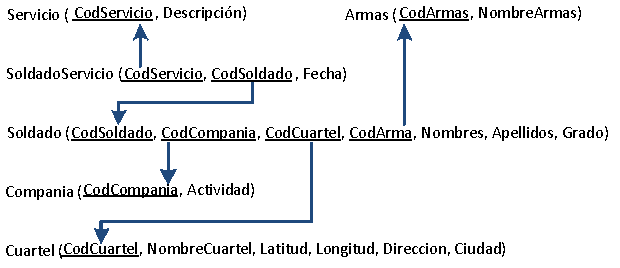
\includegraphics[width=1.0\hsize]{Relacional_Modelo/Defensa.pdf}}
        \caption{Modelo Relacional de Defensa.}
        \label{fig:Defensa_MR}
    \end{figure}
    
    \subsection{Diccionario de Datos del Modelo Relacional}
    
    \subsubsection{Dominios}
    \begin{center}
        \begin{table}[H]
    \centering
    \caption{Dominios del modelo relacional Ministerio de Defensa.}
    \renewcommand{\arraystretch}{1.5}% Spread rows out...
    \label{tab-DomR-01}
    \resizebox{1.25\textwidth}{!}{
        \begin{tabular}
            {>{\bfseries}m{2.0cm} >{\centering}m{2cm} >{}m{4cm} >{\arraybackslash}m{2cm}>{\arraybackslash}m{1cm}>{\arraybackslash}m{5cm}>{\arraybackslash}m{2cm}}
            \toprule
            \multicolumn{1}{c}{\textbf{Nombre}} & \multicolumn{1}{c}{\textbf{Tipo}} & \multicolumn{1}{c}{\textbf{Formato}} & \multicolumn{1}{c}{\textbf{Unidad}} & \multicolumn{1}{c}{\textbf{Valores}} & \multicolumn{1}{c}{\textbf{Descripción}} &
            \multicolumn{1}{c}{\textbf{Atributos}}\\ \midrule
            DCodigo     & VARCHAR             & \{Dígitos, Letras\}1,10              &                                     &                                      & Identificador Principal    &   CodArmas \newline CodServicio \newline CodSoldado \newline CodCompania \newline CodCuartel   \\\hline
            DLatitud    & NUMBER          & \{Dígitos\}                          & Grados Decimales                    & --90 a 90                            & Grados decimales con respecto al Ecuador     & Latitud           \\\hline
            DLongitud   & NUMBER          & \{Dígitos\}                          & Grados Decimales                    & --180 a 180                          & Grados decimales con respecto al meridiano de Greenwich & Longitud \\\hline
            DNombre     & VARCHAR             & \{Dígitos, Letras\}1,100             &                                     &                                      & Nombre de persona o institución     & Descripcion \newline NombreArmas \newline Nombres \newline Apellidos \newline Grado \newline Actividad \newline NombreCuartel                     \\\hline
            DDireccion  & VARCHAR             & \{Dígitos, Letras\}1,250             &                                     &                                      & Ubicación de la institución   & Direccion                          \\\hline
            DCiudad     & VARCHAR             & \{Dígitos, Letras\}1,100             &                                     &                                      & Nombre de las ciudades  & Ciudad                                \\\hline
            DFecha      & DATE             & \{dd/mm/yyyy\}                       & Fecha                               &                                      & Fecha de ejecución del servicio   & Fecha                      \\\bottomrule
        \end{tabular}
    }
\end{table}

    \end{center}
    
    \subsubsection{Entidades}
    \begin{center}
        \begin{table}[H]
\centering
\caption{Definiciones de las entidades del modelo relacional de Defensa.}
\renewcommand{\arraystretch}{1.5}% Spread rows out...
\label{tab-DiccR-00}
\begin{tabular}{>{\bfseries}m{5cm}>{}m{15cm}}
\toprule
\textbf{Entidad}  & \textbf{Definición}\\ \midrule
Armas    & Agrupador de Soldados que se encuentran en compañías y Cuarteles. \\
Cuartel  & Espacio físico donde se concentran varias armas, compañías y Soldados.\\
Compania & Ente que agrupa soldados de diversas armas.\\
Servicio & Actividad que realiza un soldado en un momento dado.\\
Soldado  & Persona que presta un servicio militar en un arma, compañía, cuartel.\\ 
SoldadoServicio & Un soldado presta uno o muchos servicios en una fecha determinada y un servicio es prestado por uno o más soldados.\\
\bottomrule
\end{tabular}
\end{table}

%Diccionario de datos de la Entidad Armas
\begin{table}[H]
\centering
\caption{Diccionario de datos de la Entidad Relacional Armas.}
\label{tab-DiccR-01}
\begin{tabular}{>{\bfseries}m{4.0cm}>{}m{3.0cm}>{}m{6.0cm}>{}m{5.0cm}>{}m{2.0cm}}
\toprule
\multicolumn{1}{c}{\textbf{Atributo}} & \multicolumn{1}{c}{\textbf{Dominio}} & \multicolumn{1}{c}{\textbf{Descripción}} & \multicolumn{1}{c}{\textbf{Defecto}} & \multicolumn{1}{c}{\textbf{Restricciones}} \\ \midrule
CodArmas    & DCodigo   & Código de identificación de las armas &   & No Nulo, Único\\
NombreArmas & DNombre   & Nombre de las armas del Ejercito  &   & No Nulo\\ \bottomrule
\end{tabular}
\end{table}

%Diccionario de datos de la Entidad Cuartel
\begin{table}[H]
\centering
\caption{Diccionario de datos de la Entidad Relacional Cuartel.}
\label{tab-DiccR-02}
\begin{tabular}{>{\bfseries}m{4.0cm}>{}m{3.0cm}>{}m{6.0cm}>{}m{5.0cm}>{}m{2.0cm}}
\toprule
\multicolumn{1}{c}{\textbf{Atributo}} & \multicolumn{1}{c}{\textbf{Dominio}} & \multicolumn{1}{c}{\textbf{Descripción}} & \multicolumn{1}{c}{\textbf{Defecto}} & \multicolumn{1}{c}{\textbf{Restricciones}} \\ \midrule
CodCuartel	    &   DCodigo	    &   Código de identificación del Cuartel	    &	&No Nulo, Único	\\
NombreCuartel	&   DNombre	    &   Nombre del Cuartel	                        &	&No Nulo	\\
Latitud	        &   Dlatitud	&   Latitud del cuartel en grados decimales	    &	&No Nulo	\\
Longitud	    &   DLongitud	&   Longitud del cuartel en grados decimales	&	&No Nulo	\\
Direccion	    &   DDireccion	&   Dirección del Cuartel	                    &	&No Nulo	\\
Ciudad	        &   DCiudad	    &   Ciudad donde está ubicado el Cuartel	    &	&No Nulo	\\\bottomrule
\end{tabular}
\end{table}

%Diccionario de datos de la Entidad Compañia
\begin{table}[H]
\centering
\caption{Diccionario de datos de la Entidad Relacional Compania.}
\label{tab-DiccR-03}
\begin{tabular}{>{\bfseries}m{4.0cm}>{}m{3.0cm}>{}m{6.0cm}>{}m{5.0cm}>{}m{2.0cm}}
\toprule
\multicolumn{1}{c}{\textbf{Atributo}} & \multicolumn{1}{c}{\textbf{Dominio}} & \multicolumn{1}{c}{\textbf{Descripción}} & \multicolumn{1}{c}{\textbf{Defecto}} & \multicolumn{1}{c}{\textbf{Restricciones}} \\ \midrule
CodCompania	    &   DCodigo	    &   Código de Identificación de la Compañía	        &	&No Nulo, Único	\\
Actividad	&   DNombre	    &   Actividad de la Compañía	                        &	&No Nulo	\\\bottomrule
\end{tabular}
\end{table}

%Diccionario de datos de la Entidad Servicio
\begin{table}[H]
\centering
\caption{Diccionario de datos de la Entidad Relacional Servicio.}
\label{tab-DiccR-04}
\begin{tabular}{>{\bfseries}m{4.0cm}>{}m{3.0cm}>{}m{6.0cm}>{}m{5.0cm}>{}m{2.0cm}}
\toprule
\multicolumn{1}{c}{\textbf{Atributo}} & \multicolumn{1}{c}{\textbf{Dominio}} & \multicolumn{1}{c}{\textbf{Descripción}} & \multicolumn{1}{c}{\textbf{Defecto}} & \multicolumn{1}{c}{\textbf{Restricciones}} \\ \midrule
CodServicio	    &   DCodigo	    &   Código de Identificación del Servicio	        &	&No Nulo, Único	\\
Descripcion	    &   DNombre	    &   Nombre del Servicio	                            &	&No Nulo	\\\bottomrule
\end{tabular}
\end{table}

%Diccionario de datos de la Entidad Soldado
\begin{table}[H]
\centering
\caption{Diccionario de datos de la Entidad Relacional Soldado.}
\label{tab-DiccR-05}
\begin{tabular}{>{\bfseries}m{4.0cm}>{}m{3.0cm}>{}m{6.0cm}>{}m{5.0cm}>{}m{2.0cm}}
\toprule
\multicolumn{1}{c}{\textbf{Atributo}} & \multicolumn{1}{c}{\textbf{Dominio}} & \multicolumn{1}{c}{\textbf{Descripción}} & \multicolumn{1}{c}{\textbf{Defecto}} & \multicolumn{1}{c}{\textbf{Restricciones}} \\ \midrule
CodSoldado	    &   DCodigo	    &   Código de identificación del Soldado	    &	&No Nulo, Único	\\
CodCompania	    &   DCodigo	    &   Código de identificación de la Compañia	    &	&No Nulo, Único	\\
CodCuartel	    &   DCodigo	    &   Código de identificación del Cuartel	    &	&No Nulo, Único	\\
CodArma	    &   DCodigo	    &   Código de identificación de la Arma &	&No Nulo, Único	\\
Nombres	        &   DNombre	    &   Nombres del Soldado	        &	&No Nulo	\\
Apellidos       &   DNombre	    &   Apellidos del Soldado	    &	&No Nulo	\\
Grado	        &   	        &   Grado del Soldado	        &	&No Nulo	\\\bottomrule
\end{tabular}
\end{table}

%Diccionario de datos de la Entidad SoldadoServicio
\begin{table}[H]
\centering
\caption{Diccionario de datos de la Entidad Relacional SoldadoServicio.}
\label{tab-DiccR-06}
\begin{tabular}{>{\bfseries}m{4.0cm}>{}m{3.0cm}>{}m{6.0cm}>{}m{5.0cm}>{}m{2.0cm}}
\toprule
\multicolumn{1}{c}{\textbf{Atributo}} & \multicolumn{1}{c}{\textbf{Dominio}} & \multicolumn{1}{c}{\textbf{Descripción}} & \multicolumn{1}{c}{\textbf{Defecto}} & \multicolumn{1}{c}{\textbf{Restricciones}} \\ \midrule
CodSoldado    & DCodigo   & Código de Identificación del Servicio &   & No Nulo, Único\\
CodServicio & DCodigo   & Código de identificación del Soldado.  &   & No Nulo, Único\\ 
Fecha & DFecha   & Fecha en que un Soldado presto un Servicio.  &   & No Nulo\\ \bottomrule
\end{tabular}
\end{table}

    \end{center}
    
    \end{landscape}
}

\newpage
%%%%%       OLIMPICOS
\section{Eventos Olímpicos}

Se solicita diseñar el modelo entidad relación para tener el control de los eventos realizados durante los eventos olímpicos, teniendo en cuenta las instalaciones y tipo donde se realizarán:
\begin{itemize}  
\item Las sedes olímpicas se dividen en complejos deportivos.
\item Los complejos deportivos se subdividen en aquellos en los que se desarrolla un único deporte y en los polideportivos.
\item Los complejos polideportivos tienen áreas designadas para cada deporte con un indicador de localización (orientación dentro del complejo, subdivisión por cuadrantes dentro del complejo para su ubicación interna, al igual que un código de identificación dentro de este).
\item Un complejo tiene una localización definido por un par de coordenadas geográficas, un jefe de organización individual y un área total ocupada.
\item Los dos tipos de complejos tendrán diferentes tipos de información. Para cada tipo de sede, se conservará el número de complejos junto con su presupuesto aproximado.
\item Cada complejo celebra una serie de eventos. Para cada evento está prevista una fecha, duración, número de participantes, número de comisarios.
\item Una lista de todos los comisarios se conservará junto con la lista de los eventos en los que esté involucrado cada comisario ya sea cumpliendo la tarea de juez u observador.
\item Para cada evento se necesitará cierto equipamiento (elementos deportivos a utilizar como jabalina, balones,...). \ldots 
\end{itemize}

\afterpage{
\begin{landscape}
    \subsection{Modelo Entidad Relación}
    
    \begin{center}
        \begin{figure}[H]
   \centering
    \begin{adjustbox}{max width=1.1\textwidth}
        \begin{tikzpicture} 
          % Entidades - Relaciones
          \matrix[row sep=3cm, column sep=4cm] {
            
            \entity{uni}{UniDeportivo} & 
            \relationship{rel_1}{Pertenece}     
            
            \\
            
            \relationship{rel_2}{Pertenece} & 
            \entity{complejo}{ComplejoDeportivo} & 
            \relationship{rel_3}{Se Realiza} 
            
            \\
            
            \entity{polidepor}{Polideportivo} & 
            \relationship{rel_4}{Posee} & 
            \entity{evento}{Evento} & 
            \relationship{rel_6}{Involucra} 
            
            \\
            
            \relationship{rel_5}{Conforma} &  &
            \relationship{rel_7}{Requiere} 
            
            \\
            
            \entity{area}{Area} & 
            \entity{sede}{SedeOlimpica} & 
            \entity{Elemento}{ElementoDeportivo}  & 
            \entity{Comisario}{Comisario} \\    
          };
          
          % relationships
          \buildrelationship{rel_1}{complejo}{(1,1)}{uni}{(1,n)}
          \buildrelationship{rel_2}{complejo}{(1,1)}{polidepor}{(1,n)}
          \buildrelationship{rel_3}{complejo}{(1,1)}{evento}{(1,n)}
          \buildrelationship{rel_4}{complejo}{(1,n)}{sede}{(1,1)}
          \buildrelationship{rel_5}{polidepor}{(1,1)}{area}{(2,n)}
          \buildrelationship{rel_6}{evento}{(1,n)}{Comisario}{(1,n)}
          \buildrelationship{rel_7}{evento}{(1,n)}{Elemento}{(1,n)}
          
          %atributos para las entidades
          %Unideporte
          \pkattrib{uni}{145}{CodComplejoUni}{35}
          \attrib{uni}{165}{Nombre}{30}
          \dvattrib{uni}{190}{Presupuesto}{30}
          \attrib{uni}{215}{Extension}{35}
          
          %Unideporte
          \pkattrib{complejo}{145}{CodComplejo}{35}
          \attrib{complejo}{70}{Jefe}{25}
          \attrib{complejo}{40}{Latitud}{30}
          \attrib{complejo}{20}{Longitud}{35}
          \attrib{complejo}{340}{Direccion}{35}
          \attrib{complejo}{310}{Ciudad}{35}
          
          %Polideportivo
          \pkattrib{polidepor}{145}{CodComplejoPoli}{35}
          \attrib{polidepor}{165}{Nombre}{30}
          \dvattrib{polidepor}{190}{Presupuesto}{30}
          \attrib{polidepor}{215}{Extension}{35}
          
          %Area
          \pkattrib{area}{145}{CodArea}{35}
          \attrib{area}{165}{Localizacion}{30}
          \attrib{area}{190}{Orientacion}{30}
          \attrib{area}{215}{Cuadrante}{35}
          \attrib{area}{260}{NombreDeporte}{30}
          \attrib{area}{310}{Extension}{30}
          
          %Sede
          \pkattrib{sede}{145}{CodSede}{35}
          \attrib{sede}{165}{Nombre}{30}
          \dvattrib{sede}{195}{Presupuesto}{30}
          \attrib{sede}{270}{NumeroComplejos}{25}
          
          %Evento
          \pkattrib{evento}{165}{CodEvento}{30}
          \attrib{evento}{195}{Fecha}{30}
          \attrib{evento}{225}{DuracionEvento}{30}
          \attrib{evento}{25}{NumeroParticipantes}{35}
          \attrib{evento}{330}{NumeroComisarios}{35}
          
          %Elemento
          \pkattrib{Elemento}{145}{CodElemento}{35}
          \attrib{Elemento}{230}{Nombre}{30}
          \attrib{Elemento}{310}{Stock}{30}
          
          %Comisario
          \pkattrib{Comisario}{230}{CodComisario}{30}
          \attrib{Comisario}{310}{Nombre}{30}
          
          \attrib{rel_6}{90}{Rol}{30}
          \attrib{rel_7}{180}{Cantidad}{30}
          
        \end{tikzpicture}
    \end{adjustbox}
    \caption{Modelo Entidad Relación de las Olimpiadas.}
    \label{fig:Olimpicos_MER}
\end{figure}
    \end{center}

    \subsection{Diccionario de Datos del Modelo Entidad Relación}
    
    \subsubsection{Dominios}
    \begin{center}
        \begin{table}[H]
\centering
\caption{Dominios del modelo ER Olimpiadas.}
\renewcommand{\arraystretch}{1.5}% Spread rows out...
\label{tab-DomER-02}
\resizebox{1.1\textwidth}{!}{
    \begin{tabular}{>{\bfseries}m{2.5cm} >{\centering}m{2cm} >{}m{4cm} >{\arraybackslash}m{2cm}>{\arraybackslash}m{2.5cm}>{\arraybackslash}m{6cm}}
    \toprule
    \multicolumn{1}{c}{\textbf{Nombre}} & \multicolumn{1}{c}{\textbf{Tipo}} & \multicolumn{1}{c}{\textbf{Formato}} & \multicolumn{1}{c}{\textbf{Unidad}} & \multicolumn{1}{c}{\textbf{Valores}} & \multicolumn{1}{c}{\textbf{Descripción}}                                                          \\ \midrule
    DCodigo     & Texto             & \{Dígitos, Letras\}1,10              &                                     &                                      & Identificador Principal                                 \\\hline
    DLatitud    & Numérico          & \{Dígitos\}                          & Grados Decimales                    & --90 a 90                            & Grados decimales con respecto al Ecuador                \\\hline
    DLongitud   & Numérico          & \{Dígitos\}                          & Grados Decimales                    & --180 a 180                          & Grados decimales con respecto al meridiano de Greenwich \\\hline
    DNombre     & Texto             & \{Dígitos, Letras\}1,100             &                                     &                                      & Nombre de persona o institución                         \\\hline
    DDireccion  & Texto             & \{Dígitos, Letras\}1,250             &                                     &                                      & Ubicación de la institución                             \\\hline
    DCiudad     & Texto             & \{Dígitos, Letras\}1,100             &                                     &                                      & Nombre de las ciudades                                  \\\hline
    
    DCantidad   & Numérico          & \{Dígitos\}                          &                                     & $ > 0$                               & Cantidad de Personas, Elementos, Comisarios, etc.       \\\hline
    DArea       & Numérico          & \{Dígitos\                           & Metros Cuadrados                    & $ > 0$                               & Área en metros cuadrados de un complejo                 \\\hline
    DDuracion   & Tiempo            & \{hh:mm\}                            & Horas -- Minutos                    &                                      & Tiempo de duración del evento                           \\\hline
    DPreupuesto & Numérico          & \{Dígitos\}1,n                       & Moneda                              &                                      & Presupuesto asignado                                    \\\hline
    DRol        & Texto             & \{Letras\}1,10                       &                                     & Juez \newline Observador             & Rol a ejecutar por un comisario                         \\\hline
    
    DFecha      & Texto             & \{dd/mm/yyyy\}                       & Fecha                               &                                      & Fecha de ejecución del servicio                         \\\bottomrule
    \end{tabular}
}
\end{table}

    \end{center}
    
    \subsubsection{Entidades}
    \begin{center}
        \begin{table}[H]
\centering
\caption{Definiciones de las entidades del modelo Entidad Relación de Olimpiadas.}
\renewcommand{\arraystretch}{1.5}% Spread rows out...
\label{tab-Dicc-10}
\begin{tabular}{@{}ll@{}}
\toprule
\textbf{Entidad}  & \textbf{Definición}\\ \midrule
Area    & Zona destinada a las actividades deportivas de un Polideportivo. \\
Comisario  & Persona encargada de observar o juzgar durante un evento deportivo.\\
ComplejoDeportivo & Espacio físico donde se realizan eventos deportivos.\\
ElementoDeportivo & Elemento, dispositivo o artefacto necesario para ejecutar un evento deportivo.\\
Evento & Actividad deportiva que se realiza en un complejo deportivo.\\
Polideportivo & Complejo donde se pueden realizar más de una actividad deportiva.\\
SedeOlimpica & Almacena los datos de la sede olímpica.\\
UniDeportivo & Complejo donde se realizar una actividad deportiva.\\ \bottomrule
\end{tabular}
\end{table}

%Diccionario de datos de la Entidad Area
\begin{table}[H]
\centering
\caption{Diccionario de datos de la Entidad Area.}
\label{tab-Dicc-11}
\begin{tabular}{>{\bfseries}m{4.0cm}>{}m{3.0cm}>{}m{6.0cm}>{}m{5.0cm}>{}m{2.0cm}}
\toprule
\multicolumn{1}{c}{\textbf{Atributo}} & \multicolumn{1}{c}{\textbf{Dominio}} & \multicolumn{1}{c}{\textbf{Descripción}} & \multicolumn{1}{c}{\textbf{Defecto}} & \multicolumn{1}{c}{\textbf{Restricciones}} \\ \midrule
CodArea    & DCodigo   & Código de Identificación  del Área deportiva &   & No Nulo, Único\\
Localizacion    & DNombre   & Localización del área dentro del polideportivo &   & No Nulo\\
Orientacion    & DNombre   & Orientación  del área dentro del polideportivo &   & No Nulo\\
Cuadrante    & DNombre   & Cuadrante del área dentro del polideportivo &   & No Nulo\\
NombreDeporte    & DNombre   & Nombre del deporte ejecutado en el área dentro del polideportivo &   & No Nulo\\
Extension & DArea   & Tamaño en metros cuadrados del área dentro del polideportivo  &   & No Nulo\\ \bottomrule
\end{tabular}
\end{table}

%Diccionario de datos de la Entidad Comisario
\begin{table}[H]
\centering
\caption{Diccionario de datos de la Entidad Comisario.}
\label{tab-Dicc-12}
\begin{tabular}{>{\bfseries}m{4.0cm}>{}m{3.0cm}>{}m{6.0cm}>{}m{5.0cm}>{}m{2.0cm}}
\toprule
\multicolumn{1}{c}{\textbf{Atributo}} & \multicolumn{1}{c}{\textbf{Dominio}} & \multicolumn{1}{c}{\textbf{Descripción}} & \multicolumn{1}{c}{\textbf{Defecto}} & \multicolumn{1}{c}{\textbf{Restricciones}} \\ \midrule
CodComisario	&   DCodigo	&   Código de Identificación  del Comisario	&	&   No Nulo, Único  \\
Nombre	&   DNombre	&   Nombres y Apellidos del Comisario	&	&   No Nulo \\\bottomrule
\end{tabular}
\end{table}

%Diccionario de datos de la Entidad ComplejoDeportivo
\begin{table}[H]
\centering
\caption{Diccionario de datos de la Entidad ComplejoDeportivo.}
\label{tab-Dicc-13}
\begin{tabular}{>{\bfseries}m{4.0cm}>{}m{3.0cm}>{}m{6.0cm}>{}m{5.0cm}>{}m{2.0cm}}
\toprule
\multicolumn{1}{c}{\textbf{Atributo}} & \multicolumn{1}{c}{\textbf{Dominio}} & \multicolumn{1}{c}{\textbf{Descripción}} & \multicolumn{1}{c}{\textbf{Defecto}} & \multicolumn{1}{c}{\textbf{Restricciones}} \\ \midrule
CodComplejo	&	DCodigo	&	Código de identificación del Complejo Deportivo	&		&	No Nulo, Único\\
Jefe	&	DNombre	&	Nombre del Jefe encargado del Complejo deportivo	&		&	No Nulo\\
Latitud	&	DLatitud	&	Latitud del complejo deportivo en grados decimales	&		&	No Nulo\\
Longitud	&	DLongitud	&	Longitud del complejo deportivo en grados decimales	&		&	No Nulo\\
Direccion	&	DDireccion	&	Dirección del complejo deportivo	&		&	No Nulo\\
Ciudad	&	DCiudad	&	Ciudad donde está ubicado el complejo deportivo	&		&	No Nulo\\\bottomrule
\end{tabular}
\end{table}

%Diccionario de datos de la Entidad ElementoDeportivo
\begin{table}[H]
\centering
\caption{Diccionario de datos de la Entidad ElementoDeportivo.}
\label{tab-Dicc-14}
\begin{tabular}{>{\bfseries}m{4.0cm}>{}m{3.0cm}>{}m{6.0cm}>{}m{5.0cm}>{}m{2.0cm}}
\toprule
\multicolumn{1}{c}{\textbf{Atributo}} & \multicolumn{1}{c}{\textbf{Dominio}} & \multicolumn{1}{c}{\textbf{Descripción}} & \multicolumn{1}{c}{\textbf{Defecto}} & \multicolumn{1}{c}{\textbf{Restricciones}} \\ \midrule
CodElemento	&	DCodigo	&	Código de Identificación del Elemento deportivo	&		&	No Nulo, Único\\
Nombre	&	DNombre	&	Nombre del Elemento Deportivo	&		&	No Nulo\\
Stock	&	DCantidad	&	Cantidad de elementos disponibles	&		&	No Nulo\\\bottomrule
\end{tabular}
\end{table}

%Diccionario de datos de la Entidad Evento
\begin{table}[H]
\centering
\caption{Diccionario de datos de la Entidad Evento.}
\label{tab-Dicc-15}
\begin{tabular}{>{\bfseries}m{4.0cm}>{}m{3.0cm}>{}m{6.0cm}>{}m{5.0cm}>{}m{2.0cm}}
\toprule
\multicolumn{1}{c}{\textbf{Atributo}} & \multicolumn{1}{c}{\textbf{Dominio}} & \multicolumn{1}{c}{\textbf{Descripción}} & \multicolumn{1}{c}{\textbf{Defecto}} & \multicolumn{1}{c}{\textbf{Restricciones}} \\ \midrule
CodEvento	&	DCodigo	&	Código de Identificación del Evento	&		&	No Nulo, Único\\
FechaEvento	&	DFecha	&	Fecha de ejecución del evento deportivo	&		&	No Nulo\\
DuracionEvento	&	DDuracion	&	Tiempo de duración del evento deportivo	&		&	No Nulo\\
NumParticipantes	&	DCantidad	&	Cantidad de participantes en la actividad	&		&	No Nulo\\
NumComisarios	&	DCantidad	&	Cantidad de Comisarios en la actividad	&		&	No Nulo\\\bottomrule
\end{tabular}
\end{table}

%Diccionario de datos de la Entidad Polideportivo
\begin{table}[H]
\centering
\caption{Diccionario de datos de la Entidad Polideportivo.}
\label{tab-Dicc-16}
\begin{tabular}{>{\bfseries}m{4.0cm}>{}m{3.0cm}>{}m{6.0cm}>{}m{5.0cm}>{}m{2.0cm}}
\toprule
\multicolumn{1}{c}{\textbf{Atributo}} & \multicolumn{1}{c}{\textbf{Dominio}} & \multicolumn{1}{c}{\textbf{Descripción}} & \multicolumn{1}{c}{\textbf{Defecto}} & \multicolumn{1}{c}{\textbf{Restricciones}} \\ \midrule
CodComplejoPoli	&	DCodigo	&	Código de identificación del Polideportivo	&		&	No Nulo, Único\\
Nombre	&	DNombre	&	Nombre del Polideportivo	&		&	No Nulo\\
Presupuesto	&	DPresupuesto	&	Presupuesto disponible para el Polideportivo	&		&	\\
Extension	&	DArea	&	Tamaño del Polideportivo	&		&	No Nulo\\\bottomrule
\end{tabular}
\end{table}

%Diccionario de datos de la Entidad SedeOlimpica
\begin{table}[H]
\centering
\caption{Diccionario de datos de la Entidad SedeOlimpica.}
\label{tab-Dicc-17}
\begin{tabular}{>{\bfseries}m{4.0cm}>{}m{3.0cm}>{}m{6.0cm}>{}m{5.0cm}>{}m{2.0cm}}
\toprule
\multicolumn{1}{c}{\textbf{Atributo}} & \multicolumn{1}{c}{\textbf{Dominio}} & \multicolumn{1}{c}{\textbf{Descripción}} & \multicolumn{1}{c}{\textbf{Defecto}} & \multicolumn{1}{c}{\textbf{Restricciones}} \\ \midrule
CodSede	&	DCodigo	&	Código de identificación de la Sede	&		&	No Nulo\\
Nombre	&	DNombre	&	Nombre de la Sede	&		&	No Nulo\\
NumeroComplejos	&	DCantidad	&	Cantidad de Complejos de la Sede	&	Sumatoria de de la cantidad complejos deportivos	&	No Nulo\\
Presupuesto	&	DPresupuesto	&	Presupuesto asignado a la sede	&	Sumatoria de los presupuestos de los complejos deportivos	&	\\\bottomrule
\end{tabular}
\end{table}

%Diccionario de datos de la Entidad UniDeportivo
\begin{table}[H]
\centering
\caption{Diccionario de datos de la Entidad UniDeportivo.}
\label{tab-Dicc-18}
\begin{tabular}{>{\bfseries}m{4.0cm}>{}m{3.0cm}>{}m{6.0cm}>{}m{5.0cm}>{}m{2.0cm}}
\toprule
\multicolumn{1}{c}{\textbf{Atributo}} & \multicolumn{1}{c}{\textbf{Dominio}} & \multicolumn{1}{c}{\textbf{Descripción}} & \multicolumn{1}{c}{\textbf{Defecto}} & \multicolumn{1}{c}{\textbf{Restricciones}} \\ \midrule
CodComplejoUni	&	DCodigo	&	Código de identificación del complejo deportivo	&		&	No Nulo, Único\\
Nombre	&	DNombre	&	Nombres del complejo deportivo	&		&	No Nulo\\
Presupuesto	&	DPresupuesto	&	Presupuesto disponible para el complejo deportivo	&		&	\\
Extension	&	DArea	&	Tamaño del complejo deportivo	&		&	No Nulo\\\bottomrule
\end{tabular}
\end{table}
    \end{center}
    
    \subsection{Modelo Relacional}
    
    \begin{figure}[H]
        \centering
        \fbox{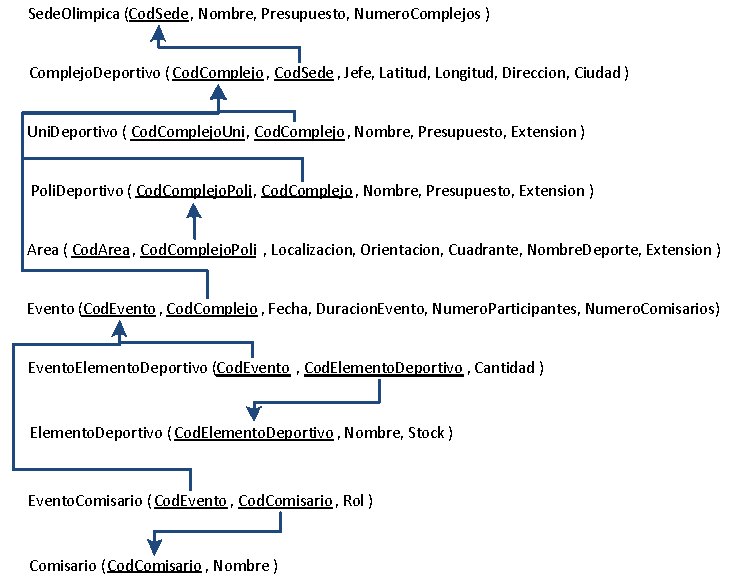
\includegraphics[width=0.75\hsize]{Relacional_Modelo/Olimpiadas.pdf}}
        \caption{Modelo Relacional de las Olimpiadas.}
        \label{fig:Olimpiadas_MR}
    \end{figure}
    
    \subsection{Diccionario de Datos del Modelo Relacional}
    
    \subsubsection{Dominios}
    \begin{center}
        \begin{table}[H]
    \centering
    \caption{Dominios del modelo relacional Olimpiadas.}
    \renewcommand{\arraystretch}{1.5}% Spread rows out...
    \label{tab-DomR-02}
    \resizebox{1.3\textwidth}{!}{
        \begin{tabular}
            {>{\bfseries}m{3.0cm} >{\centering}m{2cm} >{}m{4cm} >{\arraybackslash}m{2cm}>{\arraybackslash}m{3cm}>{\arraybackslash}m{12cm}>{\arraybackslash}m{8cm}}
            \toprule
            \multicolumn{1}{c}{\textbf{Nombre}} & \multicolumn{1}{c}{\textbf{Tipo}} & \multicolumn{1}{c}{\textbf{Formato}} & \multicolumn{1}{c}{\textbf{Unidad}} & \multicolumn{1}{c}{\textbf{Valores}} & \multicolumn{1}{c}{\textbf{Descripción}} &
            \multicolumn{1}{c}{\textbf{Atributos}}\\ \midrule
            DCodigo     & VARCHAR          & \{Dígitos, Letras\}1,10       &                   &                           & Identificador Principal                                 & ComplejoDeportivo: CodComplejo \newline  Unideportivo: CodComplejoUni \newline  Polideportivo: CodComplejoPoli \newline Evento: CodEvento \newline Area: CodArea \newline SedeOlimpica: CodSede \newline ElementoDeportivo: CodElemento \newline Comisario: CodComisario \\\hline
            DLatitud     & NUMBER          & \{Dígitos\}                   & Grados Decimales  & --90 a 90                 & Grados decimales con respecto al Ecuador                & ComplejoDeportivo: Latitud \\\hline
            DLongitud    & NUMBER          & \{Dígitos\}                   & Grados Decimales  & --180 a 180               & Grados decimales con respecto al meridiano de Greenwich & ComplejoDeportivo: Longitud \\\hline
            DNombre      & VARCHAR         & \{Dígitos, Letras\}1,100      &                   &                           & Nombre de persona o institución                         & Unideportivo: Nombre \newline ComplejoDeportivo: Jefe \newline Polideportivo: Nombre \newline SedeOlimpica: Nombre \newline ElementoDeportivo: Nombre \newline Comisario: Nombre \newline Area: NombreDeporte  \\\hline
            DDireccion   & VARCHAR         & \{Dígitos, Letras\}1,250      &                   &                           & Ubicación de la institución                             & ComplejoDeportivo: Direccion \\\hline
            DCiudad      & VARCHAR         & \{Dígitos, Letras\}1,100      &                   &                           & Nombre de las ciudades                                  & ComplejoDeportivo: Ciudad \\\hline
            DCantidad    & NUMBER          & \{Dígitos\}                   &                   & $ > 0$                    & Cantidad de Personas, Elementos, Comisarios, etc.       & SedeOlimpica: NumeroComplejos \newline Evento: NumeroParticipantes \newline Evento: NumeroComisarios \newline ElementoDeportivo: Stock \newline EventoElementoDeportivo: Cantidad \\\hline
            DArea        & NUMBER          & \{Dígitos\                    & Metros Cuadrados  & $ > 0$                    & Área en metros cuadrados de un complejo                 & Area: Extension \newline Polideportivo: Extension \newline Unideportivo: Extension \\\hline
            DDuracion    & TIME            & \{hh:mm\}                     & Horas -- Minutos  &                           & Tiempo de duración del evento                           & Evento: DuracionEvento \\\hline
            DPresupuesto & NUMBER          & \{Dígitos\}1,n                & Moneda            &                           & Presupuesto asignado                                    & Unideportivo: Presupuesto \newline Polideportivo: Presupuesto \newline SedeOlimpica: Presupuesto \\\hline
            DRol         & VARCHAR         & \{Letras\}1,10                &                   & Juez \newline Observador  & Rol a ejecutar por un comisario                         & EventoComisario: Rol \\\hline
            DFecha       & DATE             & \{dd/mm/yyyy\}                & Fecha             &                           & Fecha de ejecución del servicio                         & Evento: Fecha \\
            \bottomrule
        \end{tabular}
    }
\end{table}

    \end{center}
    
    \subsubsection{Entidades}
    \begin{center}
        \begin{table}[H]
\centering
\caption{Definiciones de las entidades del modelo relacional de Olimpiadas.}
\renewcommand{\arraystretch}{1.5}% Spread rows out...
\label{tab-DiccR-1a}
\begin{tabular}{@{}ll@{}}
\toprule
\textbf{Entidad}  & \textbf{Definición}\\ \midrule
Area    & Zona destinada a las actividades deportivas de un Polideportivo. \\
Comisario  & Persona encargada de observar o juzgar durante un evento deportivo.\\
ComplejoDeportivo & Espacio físico donde se realizan eventos deportivos.\\
ElementoDeportivo & Elemento, dispositivo o artefacto necesario para ejecutar un evento deportivo.\\
Evento & Actividad deportiva que se realiza en un complejo deportivo.\\
Polideportivo & Complejo donde se pueden realizar más de una actividad deportiva.\\
SedeOlimpica & Almacena los datos de la sede olímpica.\\
UniDeportivo & Complejo donde se realizar una actividad deportiva.\\ 
EventoElementoDeportivo & Determina la cantidad necesaria de elementos deportivos requeridos por un evento. \\
EventoComisario & Determina el rol (Juez, Observador) que realiza un comisario en un evento. \\
\bottomrule
\end{tabular}
\end{table}

%Diccionario de datos de la Entidad Area
\begin{table}[H]
\centering
\caption{Diccionario de datos de la Entidad relacional Area.}
\label{tab-DiccR-1b}
\begin{tabular}{>{\bfseries}m{4.0cm}>{}m{3.0cm}>{}m{6.0cm}>{}m{5.0cm}>{}m{2.0cm}}
\toprule
\multicolumn{1}{c}{\textbf{Atributo}} & \multicolumn{1}{c}{\textbf{Dominio}} & \multicolumn{1}{c}{\textbf{Descripción}} & \multicolumn{1}{c}{\textbf{Defecto}} & \multicolumn{1}{c}{\textbf{Restricciones}} \\ \midrule
CodArea    & DCodigo   & Código de Identificación  del Área deportiva &   & No Nulo, Único\\
CodComplejoPoli    & DCodigo   & Código de Identificación  del Polideportivo &   & No Nulo, Único\\
Localizacion    & DNombre   & Localización del área dentro del polideportivo &   & No Nulo\\
Orientacion    & DNombre   & Orientación  del área dentro del polideportivo &   & No Nulo\\
Cuadrante    & DNombre   & Cuadrante del área dentro del polideportivo &   & No Nulo\\
NombreDeporte    & DNombre   & Nombre del deporte ejecutado en el área dentro del polideportivo &   & No Nulo\\
Extension & DArea   & Tamaño en metros cuadrados del área dentro del polideportivo  &   & No Nulo\\ \bottomrule
\end{tabular}
\end{table}

%Diccionario de datos de la Entidad Comisario
\begin{table}[H]
\centering
\caption{Diccionario de datos de la Entidad relacional Comisario.}
\label{tab-DiccR-1c}
\begin{tabular}{>{\bfseries}m{4.0cm}>{}m{3.0cm}>{}m{6.0cm}>{}m{5.0cm}>{}m{2.0cm}}
\toprule
\multicolumn{1}{c}{\textbf{Atributo}} & \multicolumn{1}{c}{\textbf{Dominio}} & \multicolumn{1}{c}{\textbf{Descripción}} & \multicolumn{1}{c}{\textbf{Defecto}} & \multicolumn{1}{c}{\textbf{Restricciones}} \\ \midrule
CodComisario	&   DCodigo	&   Código de Identificación  del Comisario	&	&   No Nulo, Único  \\
Nombre	&   DNombre	&   Nombres y Apellidos del Comisario	&	&   No Nulo \\\bottomrule
\end{tabular}
\end{table}

%Diccionario de datos de la Entidad ComplejoDeportivo
\begin{table}[H]
\centering
\caption{Diccionario de datos de la Entidad relacional ComplejoDeportivo.}
\label{tab-DiccR-1d}
\begin{tabular}{>{\bfseries}m{4.0cm}>{}m{3.0cm}>{}m{6.0cm}>{}m{5.0cm}>{}m{2.0cm}}
\toprule
\multicolumn{1}{c}{\textbf{Atributo}} & \multicolumn{1}{c}{\textbf{Dominio}} & \multicolumn{1}{c}{\textbf{Descripción}} & \multicolumn{1}{c}{\textbf{Defecto}} & \multicolumn{1}{c}{\textbf{Restricciones}} \\ \midrule
CodComplejo	&	DCodigo	&	Código de identificación del Complejo Deportivo	&		&	No Nulo, Único\\
CodSede    & DCodigo   & Código de Identificación  de la Sede Olímpica. &   & No Nulo, Único\\
Jefe	&	DNombre	&	Nombre del Jefe encargado del Complejo deportivo	&		&	No Nulo\\
Latitud	&	DLatitud	&	Latitud del complejo deportivo en grados decimales	&		&	No Nulo\\
Longitud	&	DLongitud	&	Longitud del complejo deportivo en grados decimales	&		&	No Nulo\\
Direccion	&	DDireccion	&	Dirección del complejo deportivo	&		&	No Nulo\\
Ciudad	&	DCiudad	&	Ciudad donde está ubicado el complejo deportivo	&		&	No Nulo\\\bottomrule
\end{tabular}
\end{table}

%Diccionario de datos de la Entidad ElementoDeportivo
\begin{table}[H]
\centering
\caption{Diccionario de datos de la Entidad relacional ElementoDeportivo.}
\label{tab-DiccR-1e}
\begin{tabular}{>{\bfseries}m{4.0cm}>{}m{3.0cm}>{}m{6.0cm}>{}m{5.0cm}>{}m{2.0cm}}
\toprule
\multicolumn{1}{c}{\textbf{Atributo}} & \multicolumn{1}{c}{\textbf{Dominio}} & \multicolumn{1}{c}{\textbf{Descripción}} & \multicolumn{1}{c}{\textbf{Defecto}} & \multicolumn{1}{c}{\textbf{Restricciones}} \\ \midrule
CodElemento	&	DCodigo	&	Código de Identificación del Elemento deportivo	&		&	No Nulo, Único\\
Nombre	&	DNombre	&	Nombre del Elemento Deportivo	&		&	No Nulo\\
Stock	&	DCantidad	&	Cantidad de elementos disponibles	&		&	No Nulo\\\bottomrule
\end{tabular}
\end{table}

%Diccionario de datos de la Entidad Evento
\begin{table}[H]
\centering
\caption{Diccionario de datos de la Entidad relacional Evento.}
\label{tab-DiccR-1f}
\begin{tabular}{>{\bfseries}m{4.0cm}>{}m{3.0cm}>{}m{6.0cm}>{}m{5.0cm}>{}m{2.0cm}}
\toprule
\multicolumn{1}{c}{\textbf{Atributo}} & \multicolumn{1}{c}{\textbf{Dominio}} & \multicolumn{1}{c}{\textbf{Descripción}} & \multicolumn{1}{c}{\textbf{Defecto}} & \multicolumn{1}{c}{\textbf{Restricciones}} \\ \midrule
CodEvento	&	DCodigo	&	Código de Identificación del Evento	&		&	No Nulo, Único\\
CodComplejo	&	DCodigo	&	Código de identificación del Complejo Deportivo	&		&	No Nulo, Único\\
FechaEvento	&	DFecha	&	Fecha de ejecución del evento deportivo	&		&	No Nulo\\
DuracionEvento	&	DDuracion	&	Tiempo de duración del evento deportivo	&		&	No Nulo\\
NumParticipantes	&	DCantidad	&	Cantidad de participantes en la actividad	&		&	No Nulo\\
NumComisarios	&	DCantidad	&	Cantidad de Comisarios en la actividad	&		&	No Nulo\\\bottomrule
\end{tabular}
\end{table}

%Diccionario de datos de la Entidad Polideportivo
\begin{table}[H]
\centering
\caption{Diccionario de datos de la Entidad relacional Polideportivo.}
\label{tab-DiccR-1g}
\begin{tabular}{>{\bfseries}m{4.0cm}>{}m{3.0cm}>{}m{6.0cm}>{}m{5.0cm}>{}m{2.0cm}}
\toprule
\multicolumn{1}{c}{\textbf{Atributo}} & \multicolumn{1}{c}{\textbf{Dominio}} & \multicolumn{1}{c}{\textbf{Descripción}} & \multicolumn{1}{c}{\textbf{Defecto}} & \multicolumn{1}{c}{\textbf{Restricciones}} \\ \midrule
CodComplejoPoli	&	DCodigo	&	Código de identificación del Polideportivo	&		&	No Nulo, Único\\
CodComplejo	&	DCodigo	&	Código de identificación del Complejo Deportivo	&		&	No Nulo, Único\\
Nombre	&	DNombre	&	Nombre del Polideportivo	&		&	No Nulo\\
Presupuesto	&	DPresupuesto	&	Presupuesto disponible para el Polideportivo	&		&	\\
Extension	&	DArea	&	Tamaño del Polideportivo	&		&	No Nulo\\\bottomrule
\end{tabular}
\end{table}

%Diccionario de datos de la Entidad SedeOlimpica
\begin{table}[H]
\centering
\caption{Diccionario de datos de la Entidad relacional SedeOlimpica.}
\label{tab-DiccR-1h}
\begin{tabular}{>{\bfseries}m{4.0cm}>{}m{3.0cm}>{}m{6.0cm}>{}m{5.0cm}>{}m{2.0cm}}
\toprule
\multicolumn{1}{c}{\textbf{Atributo}} & \multicolumn{1}{c}{\textbf{Dominio}} & \multicolumn{1}{c}{\textbf{Descripción}} & \multicolumn{1}{c}{\textbf{Defecto}} & \multicolumn{1}{c}{\textbf{Restricciones}} \\ \midrule
CodSede	&	DCodigo	&	Código de identificación de la Sede	&		&	No Nulo\\
Nombre	&	DNombre	&	Nombre de la Sede	&		&	No Nulo\\
NumeroComplejos	&	DCantidad	&	Cantidad de Complejos de la Sede	&	Sumatoria de de la cantidad complejos deportivos	&	No Nulo\\
Presupuesto	&	DPresupuesto	&	Presupuesto asignado a la sede	&	Sumatoria de los presupuestos de los complejos deportivos	&	\\\bottomrule
\end{tabular}
\end{table}

%Diccionario de datos de la Entidad UniDeportivo
\begin{table}[H]
\centering
\caption{Diccionario de datos de la Entidad relacional UniDeportivo.}
\label{tab-DiccR-1i}
\begin{tabular}{>{\bfseries}m{4.0cm}>{}m{3.0cm}>{}m{6.0cm}>{}m{5.0cm}>{}m{2.0cm}}
\toprule
\multicolumn{1}{c}{\textbf{Atributo}} & \multicolumn{1}{c}{\textbf{Dominio}} & \multicolumn{1}{c}{\textbf{Descripción}} & \multicolumn{1}{c}{\textbf{Defecto}} & \multicolumn{1}{c}{\textbf{Restricciones}} \\ \midrule
CodComplejoUni	&	DCodigo	&	Código de identificación del complejo deportivo	&		&	No Nulo, Único\\
CodComplejo	&	DCodigo	&	Código de identificación del Complejo Deportivo	&		&	No Nulo, Único\\
Nombre	&	DNombre	&	Nombres del complejo deportivo	&		&	No Nulo\\
Presupuesto	&	DPresupuesto	&	Presupuesto disponible para el complejo deportivo	&		&	\\
Extension	&	DArea	&	Tamaño del complejo deportivo	&		&	No Nulo\\\bottomrule
\end{tabular}
\end{table}

%Diccionario de datos de la Entidad EventoElementoDeportivo
\begin{table}[H]
\centering
\caption{Diccionario de datos de la Entidad relacional EventoElementoDeportivo.}
\label{tab-DiccR-1j}
\begin{tabular}{>{\bfseries}m{4.0cm}>{}m{3.0cm}>{}m{6.0cm}>{}m{5.0cm}>{}m{2.0cm}}
\toprule
\multicolumn{1}{c}{\textbf{Atributo}} & \multicolumn{1}{c}{\textbf{Dominio}} & \multicolumn{1}{c}{\textbf{Descripción}} & \multicolumn{1}{c}{\textbf{Defecto}} & \multicolumn{1}{c}{\textbf{Restricciones}} \\ \midrule
CodEvento	&	DCodigo	&	Código de identificación de la Sede	&		&	No Nulo, Único\\
CodElemento\newline Deportivo	&	DCodigo	&	Nombre de la Sede	&		&	No Nulo, Único\\
Cantidad	&	DCantidad	&	Cantidad de elementos deportivos necesarios para el evento. 	&		&	No Nulo\\
\bottomrule
\end{tabular}
\end{table}

%Diccionario de datos de la Entidad EventoComisario
\begin{table}[H]
\centering
\caption{Diccionario de datos de la Entidad relacional EventoComisario.}
\label{tab-DiccR-1k}
\begin{tabular}{>{\bfseries}m{4.0cm}>{}m{3.0cm}>{}m{6.0cm}>{}m{5.0cm}>{}m{2.0cm}}
\toprule
\multicolumn{1}{c}{\textbf{Atributo}} & \multicolumn{1}{c}{\textbf{Dominio}} & \multicolumn{1}{c}{\textbf{Descripción}} & \multicolumn{1}{c}{\textbf{Defecto}} & \multicolumn{1}{c}{\textbf{Restricciones}} \\ \midrule
CodEvento	&	DCodigo	&	Código de identificación del Evento	&		&	No Nulo, Único\\
CodComisario	&	DCodigo	&	Código de identificación del Comisario	&		&	No Nulo, Único\\
Rol	&	DRol	&	Rol desempeñado por el comisario en el evento	&		&	No Nulo\\
\bottomrule
\end{tabular}
\end{table}
    \end{center}
    
    \end{landscape}
}

\newpage
%%%%%       BANCO
\section{Policia Nacional --- Banco}

La Policía quiere crear una base de datos sobre la seguridad en algunas entidades bancarias. Para ello tiene en cuenta:
\begin{itemize} 
\item Que cada entidad bancaria se caracteriza por un código y por el domicilio de su Central definido por una dirección.
\item Que cada entidad bancaria tiene más de una sucursal que también se caracteriza por un código y por el domicilio, así como por el número de empleados de dicha sucursal.
\item Que cada sucursal contrata, según el día, algunos vigilantes, que se caracterizan por un código y edad. Un vigilante puede ser contratado por diferentes sucursales (incluso, diferentes entidades), en distintas fechas y es un dato de interés dicha fecha, así como si se ha contratado con arma o no.
\item Por otra parte, se quiere controlar a las personas que han sido detenidas por atracar las sucursales de dichas entidades. Estas personas se definen por una clave (código) y su nombre completo.
\item Alguna de estas personas están integradas en algunas bandas organizadas y por ello se desea saber a qué banda pertenecen, sin ser de interés si la banda ha participado en el delito o no. Dichas bandas se definen por un número de banda y por el número de miembros.
\item Así mismo, es interesante saber en qué fecha ha atracado cada persona una sucursal.
Evidentemente, una persona puede atracar varias sucursales en diferentes fechas, así como que una sucursal puede ser atracada por varias personas.
\item Igualmente, se quiere saber qué Juez ha estado encargado del caso, sabiendo que un individuo, por diferentes delitos, puede ser juzgado por diferentes jueces.
\item Es de interés saber, en cada delito, si la persona detenida ha sido condenada o no y de haberlo sido, cuánto tiempo pasará en la cárcel. Un Juez se caracteriza por una clave interna del juzgado, su nombre y los años de servicio.
\end{itemize}
NOTA: En ningún caso interesa saber si un vigilante ha participado en la detención de un atracador. Es importante tener la capacidad de geo posicionar las sucursales bancarias con el fin de realizar análisis de densidad de robos por zonas dentro de períodos de tiempos. Las zonas serán definidas por las localidades de la ciudad

\afterpage{
\begin{landscape}
    \subsection{Modelo Entidad Relación}
    
    \begin{center}
        \begin{figure}[H]
   \centering
    \begin{adjustbox}{max width=1.3\textwidth}
        \begin{tikzpicture} 
          % Entidades - Relaciones
          \matrix[row sep=3cm, column sep=3cm] {
            
            \entity{banco}{Banco} & 
            \relationship{rel_1}{Pertenece}     &
            \entity{sucursal}{Sucursal}
            
            \\
            \entity{vigilante}{Vigilante} & 
            \relationship{rel_2}{Cuida} & 
            \relationship{rel_3}{Atraca} &
            \entity{juez}{Juez} 
            
            \\
            
            \entity{banda}{BandaCriminal} & 
            \relationship{rel_4}{Vinculado} & 
            \entity{delincuente}{Delincuente} &
            \relationship{rel_5}{Juzga} \\
          };
          
          % relationships
          \buildrelationship{rel_1}{banco}{(1,1)}{sucursal}{(1,n)}
          \buildrelationship{rel_2}{vigilante}{(1,n)}{sucursal}{(1,n)}
          \buildrelationship{rel_3}{sucursal}{(1,n)}{delincuente}{(1,n)}
          \buildrelationship{rel_4}{delincuente}{(2,n)}{banda}{(1,1)}
          \buildrelationship{rel_5}{delincuente}{(1,n)}{juez}{(1,n)}
          
          %atributos para las entidades
          %Banco
          \pkattrib{banco}{145}{CodBanco}{35}
          \attrib{banco}{165}{Nombre}{30}
          \attrib{banco}{185}{DireccionPrincipal}{30}
          
          %Sucursal
          \pkattrib{sucursal}{145}{CodSucursal}{35}
          \attrib{sucursal}{90}{Nombre}{20}
          \attrib{sucursal}{40}{Direccion}{25}
          \attrib{sucursal}{0}{NumeroEmpleados}{35}
          
          %Delincuente
          \pkattrib{delincuente}{145}{CodDelincuente}{35}
          \attrib{delincuente}{165}{Nombre}{30}
          
          %Vigilante
          \pkattrib{vigilante}{145}{CodVigilante}{35}
          \attrib{vigilante}{165}{Nombres}{30}
          \attrib{vigilante}{190}{Apellidos}{30}
          \attrib{vigilante}{215}{Edad}{35}
          
          %BandaCriminal
          \pkattrib{banda}{165}{CodBanda}{35}
          \attrib{banda}{185}{NumeroMiembros}{35}
          \dvattrib{banda}{215}{Nombre}{35}
          
          %Juez
          \pkattrib{juez}{165}{CodJuez}{30}
          \attrib{juez}{135}{Nombre}{30}
          \attrib{juez}{75}{TiempoServicio}{25}
          
          \dvattrib{rel_5}{0}{Condenado}{30}
          \dvattrib{rel_5}{330}{TiempoCondena}{30}
          
          \attrib{rel_2}{90}{Fecha}{25}
          \attrib{rel_2}{135}{Arma}{30}
          
          \attrib{rel_3}{180}{Fecha}{25}
      
    \end{tikzpicture}
    \end{adjustbox}
    \caption{Modelo Entidad Relación de la Policía Nacional --- Bancos.}
    \label{fig:Policia_MER}
\end{figure}
    \end{center}

    \subsection{Diccionario de Datos del Modelo Entidad Relación}
    
    \subsubsection{Dominios}
    \begin{center}
        \begin{table}[H]
\centering
\caption{Dominios del modelo ER Policía Nacional --- Bancos.}
\renewcommand{\arraystretch}{1.5}% Spread rows out...
\label{tab-DomER-03}
%\begin{tabular}{@{}lllllp{4cm}@{}}%{p{2cm} p{2cm} p{4cm} p{2cm} p{1cm} p{4cm}}
\begin{tabular}{>{\bfseries}m{2.5cm} >{\centering}m{2cm} >{}m{4cm} >{\arraybackslash}m{2cm}>{\arraybackslash}m{1cm}>{\arraybackslash}m{6cm}}
\toprule
\multicolumn{1}{c}{\textbf{Nombre}} & \multicolumn{1}{c}{\textbf{Tipo}} & \multicolumn{1}{c}{\textbf{Formato}} & \multicolumn{1}{c}{\textbf{Unidad}} & \multicolumn{1}{c}{\textbf{Valores}} & \multicolumn{1}{c}{\textbf{Descripción}}                                                          \\ \midrule
DCodigo     & Texto             & \{Dígitos, Letras\}1,10              &                                     &                                      & Identificador Principal                                 \\\hline
DNombre     & Texto             & \{Dígitos, Letras\}1,100             &                                     &                                      & Nombre de persona o institución                         \\\hline
DDireccion  & Texto             & \{Dígitos, Letras\}1,250             &                                     &                                      & Ubicación de la institución                             \\\hline
DCantidad   & Numérico          & \{Dígitos\}                          &                                     & $ > 0$                               & Cantidad de Personas, años, etc.                        \\\hline
DEdad       & Numérico          & \{Dígitos\                           &                                     & $ > 0$                               & Cantidad de Años                                        \\\hline
DFecha      & Texto             & \{dd/mm/yyyy\}                       & Fecha                               &                                      & Fecha de ejecución del servicio                         \\\bottomrule
\end{tabular}
\end{table}

    \end{center}
    
    \subsubsection{Entidades}
    \begin{center}
        \begin{table}[H]
\centering
\caption{Definiciones de las entidades del modelo Entidad Relación de Policía Nacional --- Bancos.}
\renewcommand{\arraystretch}{1.5}% Spread rows out...
\label{tab-Dicc-20}
\begin{tabular}{@{}ll@{}}
\toprule
\textbf{Entidad}  & \textbf{Definición}\\ \midrule
Banco    & Entidad Bancaria Principal. \\
BandaCriminal  & Banda que agrupa a delincuentes.\\
Delincuente & Persona que asalta una sucursal bancaria.\\
Juez & Persona que Juzga a los delincuentes.\\
Sucursal & Almacena los datos básicos de la Sucursal.\\
Vigilante & Almacena los datos básicos de los vigilantes que custodian las sucursales.\\
\bottomrule
\end{tabular}
\end{table}

%Diccionario de datos de la Entidad Banco
\begin{table}[H]
\centering
\caption{Diccionario de datos de la Entidad Banco.}
\label{tab-Dicc-21}
\begin{tabular}{>{\bfseries}m{4.0cm}>{}m{3.0cm}>{}m{6.0cm}>{}m{5.0cm}>{}m{2.0cm}}
\toprule
\multicolumn{1}{c}{\textbf{Atributo}} & \multicolumn{1}{c}{\textbf{Dominio}} & \multicolumn{1}{c}{\textbf{Descripción}} & \multicolumn{1}{c}{\textbf{Defecto}} & \multicolumn{1}{c}{\textbf{Restricciones}} \\ \midrule
CodBanco	        &	DCodigo	    &	Código de Identificación del Banco	&		&	No Nulo, Único\\
Nombre	            &	DNombre	    &	Nombre del Banco	                &		&	No Nulo\\
DireccionPrincipal	&	DDireccion	&	Dirección de la Entidad	            &		&	No Nulo\\
\bottomrule
\end{tabular}
\end{table}

%Diccionario de datos de la Entidad BandaCriminal
\begin{table}[H]
\centering
\caption{Diccionario de datos de la Entidad BandaCriminal.}
\label{tab-Dicc-22}
\begin{tabular}{>{\bfseries}m{4.0cm}>{}m{3.0cm}>{}m{6.0cm}>{}m{5.0cm}>{}m{2.0cm}}
\toprule
\multicolumn{1}{c}{\textbf{Atributo}} & \multicolumn{1}{c}{\textbf{Dominio}} & \multicolumn{1}{c}{\textbf{Descripción}} & \multicolumn{1}{c}{\textbf{Defecto}} & \multicolumn{1}{c}{\textbf{Restricciones}} \\ \midrule
CodBanda	&	DCodigo	&	Código de Identificación de la Banda	&		&	No Nulo, Único\\
NumeroMiembros	&	DCantidad	&	Cantidad de Miembros de la Banda.	&		&	No Nulo\\
Nombre	&	DNombre	&	Nombre de la Banda Criminal	&		&	\\
\bottomrule
\end{tabular}
\end{table}

%Diccionario de datos de la Entidad Delincuente
\begin{table}[H]
\centering
\caption{Diccionario de datos de la Entidad Delincuente.}
\label{tab-Dicc-23}
\begin{tabular}{>{\bfseries}m{4.0cm}>{}m{3.0cm}>{}m{6.0cm}>{}m{5.0cm}>{}m{2.0cm}}
\toprule
\multicolumn{1}{c}{\textbf{Atributo}} & \multicolumn{1}{c}{\textbf{Dominio}} & \multicolumn{1}{c}{\textbf{Descripción}} & \multicolumn{1}{c}{\textbf{Defecto}} & \multicolumn{1}{c}{\textbf{Restricciones}} \\ \midrule
CodDelincuente	&	DCodigo	&	Código de Identificación del Delincuente	&		&	No Nulo, Único\\
NombreDelincuente	&	DNombre	&	Nombres completos del delincuente.	&		&	No Nulo\\
\bottomrule
\end{tabular}
\end{table}

%Diccionario de datos de la Entidad Juez
\begin{table}[H]
\centering
\caption{Diccionario de datos de la Entidad Juez.}
\label{tab-Dicc-24}
\begin{tabular}{>{\bfseries}m{4.0cm}>{}m{3.0cm}>{}m{6.0cm}>{}m{5.0cm}>{}m{2.0cm}}
\toprule
\multicolumn{1}{c}{\textbf{Atributo}} & \multicolumn{1}{c}{\textbf{Dominio}} & \multicolumn{1}{c}{\textbf{Descripción}} & \multicolumn{1}{c}{\textbf{Defecto}} & \multicolumn{1}{c}{\textbf{Restricciones}} \\ \midrule
CodJuez	&	DCodigo	&	Código de Identificación del Juez	&		&	No Nulo, Único\\
NombreJuez	&	DNombre	&	Nombre del Juez.	&		&	No Nulo\\
TiempoServicio	&	DCantidad	&	Años de Servicio del Juez	&		&	No Nulo\\
\bottomrule
\end{tabular}
\end{table}

%Diccionario de datos de la Entidad Sucursal
\begin{table}[H]
\centering
\caption{Diccionario de datos de la Entidad Sucursal.}
\label{tab-Dicc-25}
\begin{tabular}{>{\bfseries}m{4.0cm}>{}m{3.0cm}>{}m{6.0cm}>{}m{5.0cm}>{}m{2.0cm}}
\toprule
\multicolumn{1}{c}{\textbf{Atributo}} & \multicolumn{1}{c}{\textbf{Dominio}} & \multicolumn{1}{c}{\textbf{Descripción}} & \multicolumn{1}{c}{\textbf{Defecto}} & \multicolumn{1}{c}{\textbf{Restricciones}} \\ \midrule
CodSucursal	&	DCodigo	&	Código de Identificación de la Sucursal	&		&	No Nulo, Único\\
Nombre	&	DNombre	&	Nombre de la Sucursal	&		&	No Nulo\\
Direccion	&	DDireccion	&	Dirección de la Sucursal	&		&	No Nulo\\
NumeroEmpleados	&	DCantidad	&	Numero de empleados de la Sucursal	&		&	No Nulo\\
\bottomrule
\end{tabular}
\end{table}

%Diccionario de datos de la Entidad Vigilante
\begin{table}[H]
\centering
\caption{Diccionario de datos de la Entidad Vigilante.}
\label{tab-Dicc-26}
\begin{tabular}{>{\bfseries}m{4.0cm}>{}m{3.0cm}>{}m{6.0cm}>{}m{5.0cm}>{}m{2.0cm}}
\toprule
\multicolumn{1}{c}{\textbf{Atributo}} & \multicolumn{1}{c}{\textbf{Dominio}} & \multicolumn{1}{c}{\textbf{Descripción}} & \multicolumn{1}{c}{\textbf{Defecto}} & \multicolumn{1}{c}{\textbf{Restricciones}} \\ \midrule
CodVigilante	&	DCodigo	&	Código de Identificación del Vigilante	&		&	No Nulo, Unico\\
Nombres	&	DNombre	&	Nombres del Vigilante	&		&	No Nulo\\
Apellidos	&	DNombre	&	Apellidos del Vigilante	&		&	No Nulo\\
Edad	&	DEdad	&	Edad del Vigilante	&		&	No Nulo\\
\bottomrule
\end{tabular}
\end{table}


    \end{center}
    
    \subsection{Modelo Relacional}
    
    \begin{figure}[H]
        \centering
        \fbox{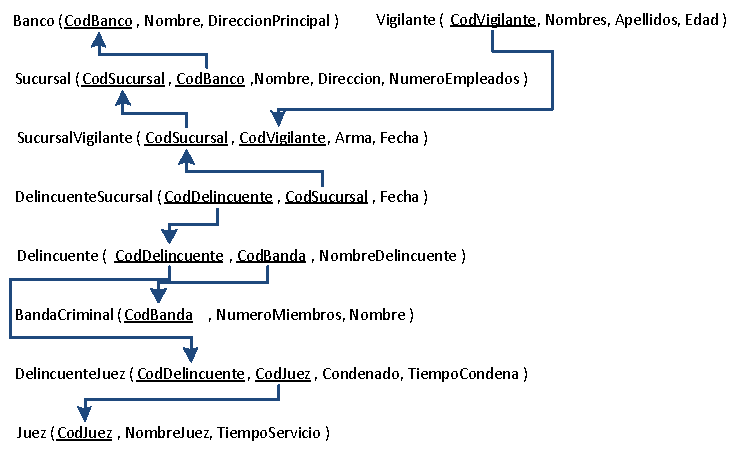
\includegraphics[width=0.9\hsize]{Relacional_Modelo/Banco.pdf}}
        \caption{Modelo Relacional de Policía Nacional --- Bancos.}
        \label{fig:Bancos_MR}
    \end{figure}
    
    \subsection{Diccionario de Datos del Modelo Relacional}
    
    \subsubsection{Dominios}
    \begin{center}
        \begin{table}[H]
    \centering
    \caption{Dominios del modelo relacional Policía Nacional --- Bancos.}
    \renewcommand{\arraystretch}{1.4}% Spread rows out...
    \label{tab-DomR-03}
    \resizebox{1.5\textwidth}{!}{
        \begin{tabular}
            {>{\bfseries}m{3.0cm} >{\centering}m{2cm} >{}m{4cm} >{\arraybackslash}m{2cm}>{\arraybackslash\centering}m{2cm}>{\arraybackslash}m{6.5cm}>{\arraybackslash}m{6.5cm}}
            \toprule
            \multicolumn{1}{c}{\textbf{Nombre}} & \multicolumn{1}{c}{\textbf{Tipo}} & \multicolumn{1}{c}{\textbf{Formato}} & \multicolumn{1}{c}{\textbf{Unidad}} & \multicolumn{1}{c}{\textbf{Valores}} & \multicolumn{1}{c}{\textbf{Descripción}} & \multicolumn{1}{c}{\textbf{Atributos}}\\ \midrule
DCodigo     & VARCHAR       & \{Dígitos, Letras\}1,10   &             &           & Identificador Principal            & Banco: CodBanco \newline Banda: CodBanda \newline Delincuente: CodDelincuente \newline Juez: CodJuez \newline Sucursal: CodSucursal \newline Vigilante: CodVigilante \\ \hline
DNombre     & VARCHAR       & \{Dígitos, Letras\}1,100  &             &           & Nombre de persona o institución    & Banco: Nombre \newline Banda: Nombre \newline Delincuente: Nombre \newline Juez: Nombre \newline Sucursal: Nombre \newline Vigilante: Nombres \newline Vigilante: Apellidos \\ \hline
DDireccion  & VARCHAR       & \{Dígitos, Letras\}1,250  &             &           & Ubicación de la institución        & Banco: Direccion \newline Sucursal: Direccion \\ \hline
DCantidad   & NUMBER        & \{Dígitos\}               &             & $ >= 0$   & Cantidad de Personas, años, etc.   & Banda: NumeroMiembros \newline Sucursal: NumeroEmpleados \\ \hline
DEdad       & NUMBER        & \{Dígitos\                &             & $ >= 0$   & Cantidad de Años                   & Juez: TiempoServicio \newline Vigilante: Edad \newline DelincuenteJuez: TiempoCondena \\ \hline
DFecha      & DATE          & \{dd/mm/yyyy\}            & Fecha       &           & Fecha de ejecución del servicio    & SucursalVigilante: Fecha \newline SucursalDelincuente: Fecha       \\ \hline
DSiNo       & VARCHAR       & \{Letras\}2               &             & SI\newline NO & Si se ha hecho o no una actividad    & SucursalVigilante: Arma \newline DelincuenteJuez: Condenado \\
            \bottomrule
        \end{tabular}
    }
\end{table}

    \end{center}
    
    \subsubsection{Entidades}
    \begin{center}
        \begin{table}[H]
\centering
\caption{Definiciones de las entidades del modelo Relacional de Policía Nacional --- Bancos.}
\renewcommand{\arraystretch}{1.5}% Spread rows out...
\label{tab-DiccR-2a}
\begin{tabular}{@{}ll@{}}
\toprule
\textbf{Entidad}  & \textbf{Definición}\\ \midrule
Banco    & Entidad Bancaria Principal. \\
BandaCriminal  & Banda que agrupa a delincuentes.\\
Delincuente & Persona que asalta una sucursal bancaria.\\
Juez & Persona que Juzga a los delincuentes.\\
Sucursal & Almacena los datos básicos de la Sucursal.\\
Vigilante & Almacena los datos básicos de los vigilantes que custodian las sucursales.\\
DelincuenteJuez & Almacena los datos del Juez que esta juzgando a un delincuente.\\
DelincuenteSucursal & Almacena los datos del delincuente que asalta una sucursal y en que fecha.\\
SucursalVigilante & Almacena los datos del vigilante que custodia una sucursal.\\

\bottomrule
\end{tabular}
\end{table}

%Diccionario de datos de la Entidad Banco
\begin{table}[H]
\centering
\caption{Diccionario de datos de la Entidad Relacional Banco.}
\label{tab-DiccR-2b}
\begin{tabular}{>{\bfseries}m{4.0cm}>{}m{3.0cm}>{}m{6.0cm}>{}m{5.0cm}>{}m{2.0cm}}
\toprule
\multicolumn{1}{c}{\textbf{Atributo}} & \multicolumn{1}{c}{\textbf{Dominio}} & \multicolumn{1}{c}{\textbf{Descripción}} & \multicolumn{1}{c}{\textbf{Defecto}} & \multicolumn{1}{c}{\textbf{Restricciones}} \\ \midrule
CodBanco	        &	DCodigo	    &	Código de Identificación del Banco	&		&	No Nulo, Único\\
Nombre	            &	DNombre	    &	Nombre del Banco	                &		&	No Nulo\\
DireccionPrincipal	&	DDireccion	&	Dirección de la Entidad	            &		&	No Nulo\\
\bottomrule
\end{tabular}
\end{table}

%Diccionario de datos de la Entidad BandaCriminal
\begin{table}[H]
\centering
\caption{Diccionario de datos de la Entidad Relacional BandaCriminal.}
\label{tab-DiccR-2c}
\begin{tabular}{>{\bfseries}m{4.0cm}>{}m{3.0cm}>{}m{6.0cm}>{}m{5.0cm}>{}m{2.0cm}}
\toprule
\multicolumn{1}{c}{\textbf{Atributo}} & \multicolumn{1}{c}{\textbf{Dominio}} & \multicolumn{1}{c}{\textbf{Descripción}} & \multicolumn{1}{c}{\textbf{Defecto}} & \multicolumn{1}{c}{\textbf{Restricciones}} \\ \midrule
CodBanda	&	DCodigo	&	Código de Identificación de la Banda Criminal	&		&	No Nulo, Único\\
NumeroMiembros	&	DCantidad	&	Cantidad de Miembros de la Banda.	&		&	No Nulo\\
Nombre	&	DNombre	&	Nombre de la Banda Criminal	&		&	\\
\bottomrule
\end{tabular}
\end{table}

%Diccionario de datos de la Entidad Delincuente
\begin{table}[H]
\centering
\caption{Diccionario de datos de la Entidad Relacional Delincuente.}
\label{tab-DiccR-2d}
\begin{tabular}{>{\bfseries}m{4.0cm}>{}m{3.0cm}>{}m{6.0cm}>{}m{5.0cm}>{}m{2.0cm}}
\toprule
\multicolumn{1}{c}{\textbf{Atributo}} & \multicolumn{1}{c}{\textbf{Dominio}} & \multicolumn{1}{c}{\textbf{Descripción}} & \multicolumn{1}{c}{\textbf{Defecto}} & \multicolumn{1}{c}{\textbf{Restricciones}} \\ \midrule
CodDelincuente	&	DCodigo	&	Código de Identificación del Delincuente	&		&	No Nulo, Único\\
NombreDelincuente	&	DNombre	&	Nombres completos del delincuente.	&		&	No Nulo\\
\bottomrule
\end{tabular}
\end{table}

%Diccionario de datos de la Entidad Juez
\begin{table}[H]
\centering
\caption{Diccionario de datos de la Entidad Relacional Juez.}
\label{tab-DiccR-2f}
\begin{tabular}{>{\bfseries}m{4.0cm}>{}m{3.0cm}>{}m{6.0cm}>{}m{5.0cm}>{}m{2.0cm}}
\toprule
\multicolumn{1}{c}{\textbf{Atributo}} & \multicolumn{1}{c}{\textbf{Dominio}} & \multicolumn{1}{c}{\textbf{Descripción}} & \multicolumn{1}{c}{\textbf{Defecto}} & \multicolumn{1}{c}{\textbf{Restricciones}} \\ \midrule
CodJuez	&	DCodigo	&	Código de Identificación del Juez	&		&	No Nulo, Único\\
NombreJuez	&	DNombre	&	Nombre del Juez.	&		&	No Nulo\\
TiempoServicio	&	DCantidad	&	Años de Servicio del Juez	&		&	No Nulo\\
\bottomrule
\end{tabular}
\end{table}

%Diccionario de datos de la Entidad Sucursal
\begin{table}[H]
\centering
\caption{Diccionario de datos de la Entidad Relacional Sucursal.}
\label{tab-DiccR-2g}
\begin{tabular}{>{\bfseries}m{4.0cm}>{}m{3.0cm}>{}m{6.0cm}>{}m{5.0cm}>{}m{2.0cm}}
\toprule
\multicolumn{1}{c}{\textbf{Atributo}} & \multicolumn{1}{c}{\textbf{Dominio}} & \multicolumn{1}{c}{\textbf{Descripción}} & \multicolumn{1}{c}{\textbf{Defecto}} & \multicolumn{1}{c}{\textbf{Restricciones}} \\ \midrule
CodSucursal	&	DCodigo	&	Código de Identificación de la Sucursal	&		&	No Nulo, Único\\
CodBanco	&	DCodigo	&	Código de Identificación del Banco	&		&	No Nulo, Único\\
Nombre	&	DNombre	&	Nombre de la Sucursal	&		&	No Nulo\\
Direccion	&	DDireccion	&	Dirección de la Sucursal	&		&	No Nulo\\
NumeroEmpleados	&	DCantidad	&	Numero de empleados de la Sucursal	&		&	No Nulo\\
\bottomrule
\end{tabular}
\end{table}

%Diccionario de datos de la Entidad Vigilante
\begin{table}[H]
\centering
\caption{Diccionario de datos de la Entidad Relacional Vigilante.}
\label{tab-DiccR-2h}
\begin{tabular}{>{\bfseries}m{4.0cm}>{}m{3.0cm}>{}m{6.0cm}>{}m{5.0cm}>{}m{2.0cm}}
\toprule
\multicolumn{1}{c}{\textbf{Atributo}} & \multicolumn{1}{c}{\textbf{Dominio}} & \multicolumn{1}{c}{\textbf{Descripción}} & \multicolumn{1}{c}{\textbf{Defecto}} & \multicolumn{1}{c}{\textbf{Restricciones}} \\ \midrule
CodVigilante	&	DCodigo	&	Código de Identificación del Vigilante	&		&	No Nulo, Único\\
Nombres	&	DNombre	&	Nombres del Vigilante	&		&	No Nulo\\
Apellidos	&	DNombre	&	Apellidos del Vigilante	&		&	No Nulo\\
Edad	&	DEdad	&	Edad del Vigilante	&		&	No Nulo\\
\bottomrule
\end{tabular}
\end{table}

%Diccionario de datos de la Entidad DelincuenteJuez
\begin{table}[H]
\centering
\caption{Diccionario de datos de la Entidad Relacional DelincuenteJuez.}
\label{tab-DiccR-2i}
\begin{tabular}{>{\bfseries}m{4.0cm}>{}m{3.0cm}>{}m{6.0cm}>{}m{5.0cm}>{}m{2.0cm}}
\toprule
\multicolumn{1}{c}{\textbf{Atributo}} & \multicolumn{1}{c}{\textbf{Dominio}} & \multicolumn{1}{c}{\textbf{Descripción}} & \multicolumn{1}{c}{\textbf{Defecto}} & \multicolumn{1}{c}{\textbf{Restricciones}} \\ \midrule
CodDelincuente	&	DCodigo	&	Código de Identificación del Delincuente	&		&	No Nulo, Único\\
CodJuez	&	DCodigo	&	Código de Identificación del Juez	&		&	No Nulo, Único\\
Condenado	&	DSiNo	&	Almacena si el delincuente recibió o no una condena	&		&	\\
TiempoCondena	&	DCantidad	&	Almacena el tiempo (en meses) de la condena del delincuente.	&		&	\\
\bottomrule
\end{tabular}
\end{table}

%Diccionario de datos de la Entidad DelincuenteSucursal
\begin{table}[H]
\centering
\caption{Diccionario de datos de la Entidad Relacional DelincuenteSucursal.}
\label{tab-DiccR-2j}
\begin{tabular}{>{\bfseries}m{4.0cm}>{}m{3.0cm}>{}m{6.0cm}>{}m{5.0cm}>{}m{2.0cm}}
\toprule
\multicolumn{1}{c}{\textbf{Atributo}} & \multicolumn{1}{c}{\textbf{Dominio}} & \multicolumn{1}{c}{\textbf{Descripción}} & \multicolumn{1}{c}{\textbf{Defecto}} & \multicolumn{1}{c}{\textbf{Restricciones}} \\ \midrule
CodDelincuente	&	DCodigo	&	Código de Identificación del Delincuente	&		&	No Nulo, Único\\
CodSucursal	&	DCodigo	&	Código de Identificación de la Sucursal	&		&	No Nulo, Único\\
Fecha	&	DFecha	&	Fecha en que se produjo el atraco	&		&	No Nulo \\
\bottomrule
\end{tabular}
\end{table}

%Diccionario de datos de la Entidad SucursalVigilante
\begin{table}[H]
\centering
\caption{Diccionario de datos de la Entidad Relacional SucursalVigilante.}
\label{tab-DiccR-2k}
\begin{tabular}{>{\bfseries}m{4.0cm}>{}m{3.0cm}>{}m{6.0cm}>{}m{5.0cm}>{}m{2.0cm}}
\toprule
\multicolumn{1}{c}{\textbf{Atributo}} & \multicolumn{1}{c}{\textbf{Dominio}} & \multicolumn{1}{c}{\textbf{Descripción}} & \multicolumn{1}{c}{\textbf{Defecto}} & \multicolumn{1}{c}{\textbf{Restricciones}} \\ \midrule
CodSucursal	&	DCodigo	&	Código de Identificación de la Sucursal	&		&	No Nulo, Único\\
CodVigilante	&	DCodigo	&	Código de Identificación del Vigilante	&		&	No Nulo, Único\\
Arma	&	DSiNo	&	Almacena si el servicio fue prestado con o sin arma.	&		&	No Nulo \\
Fecha	&	DFecha	&	Almacena la fecha en la que se presta el servicio.	&		& No Nulo	\\
\bottomrule
\end{tabular}
\end{table}
    \end{center}
    
    \end{landscape}
}

\newpage
%%%%%       CLUB NAUTICO
\section{Club Náutico}

Un club náutico desea tener informatizados los datos correspondientes a sus instalaciones, empleados, socios y embarcaciones que se encuentran en dicho club. El club está organizado de la siguiente forma:
\begin{itemize}
    \item Los socios pertenecientes al club vienen definidos por su nombre, dirección, CC, teléfono y fecha de ingreso en el club.
    \item Las embarcaciones vienen definidas por: matricula, nombre, tipo y dimensiones.
    \item Los amarres tienen como datos de interés el número de amarre, la lectura del contador de agua y luz, y si tienen o no servicios de mantenimiento contratados.
    \item Por otro lado, hay que tener en cuenta que una embarcación pertenece a un socio aunque un socio puede tener varias embarcaciones. Una embarcación ocupará un amarre y un amarre está ocupado por una sola embarcación. Es importante la fecha en la que una embarcación es asignada a un amarre.
    \item Los socios pueden ser propietarios de amarres, siendo importante la fecha de compra del amarre. Hay que tener en cuenta que un amarre pertenece a un solo socio y que NO HAY ninguna relación directa entre la fecha en la que se compra un amarre y en la que una embarcación se asigna a un amarre.
    \item El club náutico está dividido en varias zonas definidas por una letra, el tipo de barcos que tiene, el número de barcos que contiene, la profundidad y el ancho de los amarres. Una zona tendrá varios amarres y un amarre pertenece a una sola zona.
    \item En cuanto a los empleados, estos vienen definidos por su código, nombre, dirección, teléfono y especialidad. Un empleado está asignado a varias zonas y en una zona puede haber más de un empleado, siendo de interés el número de barcos de los que se encarga en cada zona. Hay que tener en cuenta que un empleado puede no encargarse de todos los barcos de una zona.
\end{itemize}

\afterpage{
\begin{landscape}
    \subsection{Modelo Entidad Relación}
    
    \begin{center}
        \begin{figure}[H]
   \centering
    \begin{adjustbox}{max width=1.1\textwidth}
        \begin{tikzpicture} 

              \matrix[row sep=3cm, column sep=3cm] {
                
                \entity{emp}{Empleado} \\
                
                \relationship{rel_1}{Atiende}     &
                \entity{zona}{Zona}         &
                \relationship{rel_2}{Pertenece} 
                
                \\
                \entity{socio}{Socio} & 
                \relationship{rel_3}{Posee} &
                \entity{amarre}{Amarre} 
                
                \\
                
                \relationship{rel_4}{Propietario} & 
                \entity{emb}{Embarcacion} &
                \relationship{rel_5}{Ocupa}  \\    
              };
              
              % relationships
              \buildrelationship{rel_1}{emp}{(1,n)}{zona}{(2,n)}
              \buildrelationship{rel_2}{zona}{(1,1)}{amarre}{(2,n)}
              \buildrelationship{rel_3}{amarre}{(0,n)}{socio}{(0,1)}
              \buildrelationship{rel_4}{socio}{(1,1)}{emb}{(1,n)}
              \buildrelationship{rel_5}{emb}{(0,1)}{amarre}{(1,1)}
              
              %atributos para las entidades
              %Unideporte
              \pkattrib{emp}{180}{CodEmpleado}{30}
              \attrib{emp}{210}{Nombres}{35}
              \attrib{emp}{240}{Apellidos}{30}
              \mvattrib{emp}{0}{Especialidad}{30}
              \attrib{emp}{-25}{Direccion}{35}
              \mvattrib{emp}{-45}{Telefonos}{35}
              
              %Unideporte
              \pkattrib{zona}{90}{CodZona}{25}
              \attrib{zona}{50}{Letra}{25}
              \attrib{zona}{20}{Profundidad}{35}
              \attrib{zona}{-20}{Ancho}{25}
              \attrib{zona}{-45}{TipoBarcos}{25}
              \attrib{zona}{-90}{CantidadBarcos}{25}
              
              %Polideportivo
              \pkattrib{socio}{90}{CodSocio}{15}
              \attrib{socio}{145}{Cedula}{25}
              \attrib{socio}{165}{Nombres}{30}
              \attrib{socio}{185}{Apellidos}{30}
              \attrib{socio}{205}{Direccion}{30}
              \mvattrib{socio}{225}{Telefonos}{30}
              \attrib{socio}{330}{FechaAfiliacion}{25}
              
              %Area
              \pkattrib{amarre}{45}{CodAmarre}{35}
              \attrib{amarre}{25}{Numero}{30}
              \attrib{amarre}{5}{Mantenimiento}{30}
              \attrib{amarre}{-15}{Agua}{35}
              \attrib{amarre}{-35}{Luz}{35}
              
              %Sede
              \pkattrib{emb}{155}{CodEmbarcacion}{30}
              \attrib{emb}{30}{Matricula}{25}
              \attrib{emb}{225}{Nombre}{20}
              \attrib{emb}{270}{Tipo}{20}
              \mvattrib{emb}{320}{Dimensiones}{23}
              
              
              \attrib{rel_1}{270}{CantidadBarcos}{15}
              \dvattrib{rel_3}{270}{FechaCompra}{20}
              
              \attrib{rel_5}{270}{FechaAsignacion}{15}
              %\attrib{rel_4}{270}{FechaCompra}{15}
      
        \end{tikzpicture}
    \end{adjustbox}
    \caption{Modelo Entidad Relación del Club Náutico.}
    \label{fig:Club_MER}
\end{figure}
    \end{center}

    \subsection{Diccionario de Datos del Modelo Entidad Relación}
    
    \subsubsection{Dominios}
    \begin{center}
        \begin{table}[H]
\centering
\caption{Dominios del modelo ER Club Náutico.}
\renewcommand{\arraystretch}{1.5}% Spread rows out...
\label{tab-DomER-04}
%\begin{tabular}{@{}lllllp{4cm}@{}}%{p{2cm} p{2cm} p{4cm} p{2cm} p{1cm} p{4cm}}
\begin{tabular}{>{\bfseries}m{2.5cm} >{\centering}m{2cm} >{}m{4cm} >{\arraybackslash}m{2cm}>{\arraybackslash}m{1cm}>{\arraybackslash}m{6cm}}
\toprule
\multicolumn{1}{c}{\textbf{Nombre}} & \multicolumn{1}{c}{\textbf{Tipo}} & \multicolumn{1}{c}{\textbf{Formato}} & \multicolumn{1}{c}{\textbf{Unidad}} & \multicolumn{1}{c}{\textbf{Valores}} & \multicolumn{1}{c}{\textbf{Descripción}}                                                          \\ \midrule
DCodigo     & Texto             & \{Dígitos, Letras\}1,10              &                                     &                                      & Identificador Principal                                 \\\hline
DNombre     & Texto             & \{Dígitos, Letras\}1,100             &                                     &                                      & Nombre de persona o institución                         \\\hline
DDireccion  & Texto             & \{Dígitos, Letras\}1,250             &                                     &                                      & Ubicación de la institución                             \\\hline

DCantidad   & Numérico          & \{Dígitos\}                          &                                     & $ > 0 $                              & Cantidad de elementos, personas                         \\\hline
DCedula     & Texto             & \{Dígitos\}1,10                      &                                     &                                      & Cédula de Ciudadanía                                    \\\hline
DTelefono   & Texto             & \{Dígitos\}1,15                      &                                     &                                      & Número de Teléfono                                      \\\hline
DTipoBarco  & Texto             & \{Letras\}1,20                       &                                     &                                      & Tipo de Barco                                           \\\hline
DDimensiones& Texto             & \{Letras\}1,50                       &                                     &                                      & Dimensiones del Banco (Ancho y largo, Calado)           \\\hline
DContrato   & Texto             & \{Letras\}1, 2                       &                                     & SI \newline NO                       & Determina si tiene contratado servicios                 \\\hline

DFecha      & Texto             & \{dd/mm/yyyy\}                       & Fecha                               &                                      & Fecha de ejecución del servicio                         \\\bottomrule
\end{tabular}
\end{table}

    \end{center}
    
    \subsubsection{Entidades}
    \begin{center}
        \begin{table}[H]
\centering
\caption{Definiciones de las entidades del modelo Entidad Relación del Club Náutico.}
\renewcommand{\arraystretch}{1.5}% Spread rows out...
\label{tab-Dicc-30}
\begin{tabular}{@{}ll@{}}
\toprule
\textbf{Entidad}  & \textbf{Definición}\\ \midrule
Amarre    & Lugar donde se deja un Bote. \\
Embarcacion  & Bote propiedad de un socio.\\
Empleado & Encargado de cuidar los botes.\\
Socio & Persona afiliada a un Club Náutico.\\
Zona & Lugar de ubicación de los amarres.\\
\bottomrule
\end{tabular}
\end{table}

%Diccionario de datos de la Entidad Amarre
\begin{table}[H]
\centering
\caption{Diccionario de datos de la Entidad Amarre.}
\label{tab-Dicc-31}
\begin{tabular}{>{\bfseries}m{4.0cm}>{}m{3.0cm}>{}m{6.0cm}>{}m{5.0cm}>{}m{2.0cm}}
\toprule
\multicolumn{1}{c}{\textbf{Atributo}} & \multicolumn{1}{c}{\textbf{Dominio}} & \multicolumn{1}{c}{\textbf{Descripción}} & \multicolumn{1}{c}{\textbf{Defecto}} & \multicolumn{1}{c}{\textbf{Restricciones}} \\ \midrule
codAmarre	&	DCodigo	&	Código de Identificación del Amarre	&		&	No Nulo, Único\\
Numero	&	Dcantidad	&	Numero del Amarre	&		&	No Nulo\\
Mantenimiento	&	Dcontrato	&	Si tiene contratado Servicios	&		&	No Nulo\\
Agua	&	DCantidad	&	Cantidad medida en el contador de Agua	&		&	No Nulo\\
Luz	&	Dcantidad	&	Cantidad medida en el contador de Luz	&		&	Nulo\\
\bottomrule
\end{tabular}
\end{table}

%Diccionario de datos de la Entidad Embarcacion
\begin{table}[H]
\centering
\caption{Diccionario de datos de la Entidad Embarcacion.}
\label{tab-Dicc-32}
\begin{tabular}{>{\bfseries}m{4.0cm}>{}m{3.0cm}>{}m{6.0cm}>{}m{5.0cm}>{}m{2.0cm}}
\toprule
\multicolumn{1}{c}{\textbf{Atributo}} & \multicolumn{1}{c}{\textbf{Dominio}} & \multicolumn{1}{c}{\textbf{Descripción}} & \multicolumn{1}{c}{\textbf{Defecto}} & \multicolumn{1}{c}{\textbf{Restricciones}} \\ \midrule
CodEmbarcacion	&	DCodigo	&	Código de Identificación del Barco	&		&	No Nulo, Único\\
Nombre	&	DNombre	&	Nombre del Barco	&		&	No Nulo\\
Matricula	&	DNombre	&	Matricula del Barco	&		&	No Nulo\\
Tipo	&	DTipoBarco	&	Tipo de Barco	&		&	No Nulo\\
Dimensiones	&	DDimensiones	&	Dimensiones del Barco	&		&	No Nulo\\
\bottomrule
\end{tabular}
\end{table}

%Diccionario de datos de la Entidad Empleado
\begin{table}[H]
\centering
\caption{Diccionario de datos de la Entidad Empleado.}
\label{tab-Dicc-33}
\begin{tabular}{>{\bfseries}m{4.0cm}>{}m{3.0cm}>{}m{6.0cm}>{}m{5.0cm}>{}m{2.0cm}}
\toprule
\multicolumn{1}{c}{\textbf{Atributo}} & \multicolumn{1}{c}{\textbf{Dominio}} & \multicolumn{1}{c}{\textbf{Descripción}} & \multicolumn{1}{c}{\textbf{Defecto}} & \multicolumn{1}{c}{\textbf{Restricciones}} \\ \midrule
CodEmpleado	&	DCodigo	&	Código de Identificación del Empleado	&		&	No Nulo, Único\\
Nombres	&	DNombre	&	Nombres del Empleado	&		&	No Nulo\\
Apellidos	&	DNombre	&	Apellidos del Empleado	&		&	No Nulo\\
Direccion	&	DDireccion	&	Dirección del Empleado	&		&	No Nulo\\
Telefono	&	DTelefono	&	Teléfono del Empleado	&		&	No Nulo\\
Especialidad	& DEspecialidad		&	Especialidad	&		&	No Nulo\\
\bottomrule
\end{tabular}
\end{table}

%Diccionario de datos de la Entidad Socio
\begin{table}[H]
\centering
\caption{Diccionario de datos de la Entidad Socio.}
\label{tab-Dicc-34}
\begin{tabular}{>{\bfseries}m{4.0cm}>{}m{3.0cm}>{}m{6.0cm}>{}m{5.0cm}>{}m{2.0cm}}
\toprule
\multicolumn{1}{c}{\textbf{Atributo}} & \multicolumn{1}{c}{\textbf{Dominio}} & \multicolumn{1}{c}{\textbf{Descripción}} & \multicolumn{1}{c}{\textbf{Defecto}} & \multicolumn{1}{c}{\textbf{Restricciones}} \\ \midrule
CodSocio	&	DCodigo	&	Código de Identificación del Socio	&		&	No Nulo, Único\\
Cedula	&	DCedula	&	Cedula del Socio	&		&	No Nulo\\
Nombres	&	Dnombre	&	Nombres del Socio	&		&	No Nulo\\
Apellidos	&	DNombre	&	Apellidos del Socio	&		&	No Nulo\\
Direccion	&	DDireccion	&	Dirección del Socio	&		&	No Nulo\\
Telefono	&	DTelefono	&	Teléfono del Socio	&		&	No Nulo\\
FechaIngreso	&	DFecha	&	Fecha de Ingreso del Socio al Club Náutico	&		&	No Nulo\\
\bottomrule
\end{tabular}
\end{table}

%Diccionario de datos de la Entidad Zona
\begin{table}[H]
\centering
\caption{Diccionario de datos de la Entidad Zona.}
\label{tab-Dicc-35}
\begin{tabular}{>{\bfseries}m{4.0cm}>{}m{3.0cm}>{}m{6.0cm}>{}m{5.0cm}>{}m{2.0cm}}
\toprule
\multicolumn{1}{c}{\textbf{Atributo}} & \multicolumn{1}{c}{\textbf{Dominio}} & \multicolumn{1}{c}{\textbf{Descripción}} & \multicolumn{1}{c}{\textbf{Defecto}} & \multicolumn{1}{c}{\textbf{Restricciones}} \\ \midrule
codZona	&	DCodigo	&	Código de Identificación de la Zona	&		&	No Nulo, Único\\
Letra	&	DLetra	&	Letra identificativa de la Zona	&		&	No Nulo\\
TipoBarco	&	DTipoBarco	&	Tipo de barcos a ubicar en la zona	&		&	No Nulo\\
NumeroBarcos	&	DCantidad	&	Numero de Barcos en la zona	&		&	No Nulo\\
Profundidad	&	DCantidad	&	Profundidad de la Zona	&		&	No Nulo\\
Ancho	&	DCantidad	&	Ancho de la Zona	&		&	No Nulo\\
\bottomrule
\end{tabular}
\end{table}

    \end{center}
    
    \subsection{Modelo Relacional}
    
    \begin{figure}[H]
        \centering
        \fbox{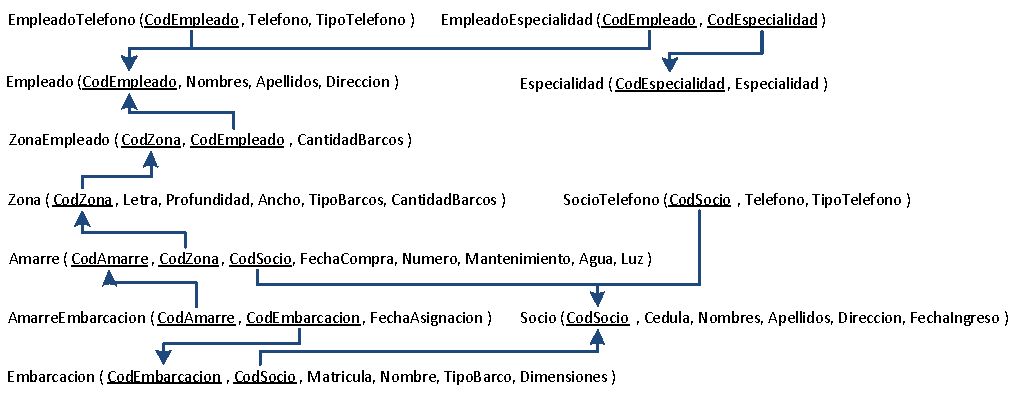
\includegraphics[width=1.0\hsize]{Relacional_Modelo/Club.pdf}}
        \caption{Modelo Relacional del Club Náutico.}
        \label{fig:Club_MR}
    \end{figure}
    
    \subsection{Diccionario de Datos del Modelo Relacional}
    
    \subsubsection{Dominios}
    \begin{center}
        \begin{table}[H]
    \centering
    \caption{Dominios del modelo relacional Club Náutico.}
    \renewcommand{\arraystretch}{1.4}% Spread rows out...
    \label{tab-DomR-04}
    \resizebox{1.4\textwidth}{!}{
        \begin{tabular}
            {>{\bfseries}m{3.0cm} >{\centering}m{2cm} >{}m{4cm} >{\arraybackslash}m{2cm}>{\arraybackslash\centering}m{2cm}>{\arraybackslash}m{9cm}>{\arraybackslash}m{7cm}}
            \toprule
            \multicolumn{1}{c}{\textbf{Nombre}} & \multicolumn{1}{c}{\textbf{Tipo}} & \multicolumn{1}{c}{\textbf{Formato}} & \multicolumn{1}{c}{\textbf{Unidad}} & \multicolumn{1}{c}{\textbf{Valores}} & \multicolumn{1}{c}{\textbf{Descripción}} & \multicolumn{1}{c}{\textbf{Atributos}}\\ \midrule
DCodigo     & VARCHAR  & \{Dígitos, Letras\}1,10   &        &                & Identificador Principal                       & Amarre: CodAmarre \newline Embarcacion: CodEmbarcacion \newline Empleado: CodEmpleado \newline Socio: CodSocio \newline Zona: CodZona \newline Especialidad: CodEspecialidad   \\ \hline
DNombre     & VARCHAR  & \{Dígitos, Letras\}1,100  &        &                & Nombre de persona o institución               & Embarcacion: Nombre \newline Embarcacion: Matricula \newline Empleado: Nombres \newline Empleado: Apellidos \newline Socio: Nombres \newline Socio: Apellidos \newline Zona: Letra        \\ \hline
DDireccion  & VARCHAR  & \{Dígitos, Letras\}1,250  &        &                & Ubicación de la institución                   & Empleado: Direccion \newline Socio: Direccion        \\ \hline
DEspecialidad & VARCHAR  & \{Dígitos, Letras\}1,100  &      &                & Especialidades en Barcos                      & Especialidad: Especialidad      \\ \hline
DCantidad   & NUMBER   & \{Dígitos\}               &        & $ >= 0 $       & Cantidad de elementos, personas               & Amarre: Numero \newline Amarre: Agua \newline Amarre: Luz \newline Zona: Profundidad \newline Zona: Ancho \newline Zona: CantidadBarcos \newline ZonaEmpleado: CantidadBarcos       \\ \hline
DCedula     & VARCHAR  & \{Dígitos\}1,10           &        &                & Cédula de Ciudadanía                          & Socio: Cedula         \\ \hline
DTelefono   & VARCHAR  & \{Dígitos\}1,15           &        &                & Número de Teléfono                            & EmpleadoTelefono: Telefono \newline SocioTelefono: Telefono         \\ \hline
DTipoBarco  & VARCHAR  & \{Letras\}1,20            &        &                & Tipo de Barco                                 & Embarcacion: Tipo \newline Zona: TipoBarcos         \\ 
            \bottomrule
        \end{tabular}
    }
\end{table}


\begin{table}[H]
    \centering
    \renewcommand{\arraystretch}{1.4}% Spread rows out...
    \resizebox{1.4\textwidth}{!}{
        \begin{tabular}
            {>{\bfseries}m{3.0cm} >{\centering}m{2cm} >{}m{4cm} >{\arraybackslash}m{2cm}>{\arraybackslash\centering}m{2cm}>{\arraybackslash}m{9cm}>{\arraybackslash}m{7cm}}
            \toprule
            \multicolumn{1}{c}{\textbf{Nombre}} & \multicolumn{1}{c}{\textbf{Tipo}} & \multicolumn{1}{c}{\textbf{Formato}} & \multicolumn{1}{c}{\textbf{Unidad}} & \multicolumn{1}{c}{\textbf{Valores}} & \multicolumn{1}{c}{\textbf{Descripción}} & \multicolumn{1}{c}{\textbf{Atributos}}\\ \midrule

DDimensiones& VARCHAR  & \{Letras\}1,50            &        &                & Dimensiones del Banco (Ancho, largo, Calado)  & Embarcacion: Dimensiones         \\ \hline
DContrato   & VARCHAR  & \{Letras\}1, 2            &        & SI \newline NO & Determina si tiene contratado servicios       & Amarre: Mantenimiento         \\ \hline

DFecha      & DATE     & \{dd/mm/yyyy\}            & Fecha  &                & Fecha de ejecución del servicio               & Socio: FechaAfiliacion \newline Amarre: FechaCompra \newline AmarreEmbarcacion: FechaAsignacion         \\
            \bottomrule
        \end{tabular}
    }
\end{table}

    \end{center}
    
    \subsubsection{Entidades}
    \begin{center}
        \begin{table}[H]
\centering
\caption{Definiciones de las entidades del modelo Relacional del Club Náutico.}
\renewcommand{\arraystretch}{1.5}% Spread rows out...
\label{tab-DiccR-3a}
\begin{tabular}{@{}ll@{}}
\toprule
\textbf{Entidad}  & \textbf{Definición}\\ \midrule
Amarre    & Lugar donde se deja un Bote. \\
Embarcacion  & Bote propiedad de un socio.\\
Empleado & Encargado de cuidar los botes.\\
Especialidad & Especialidad sobre el cuidado de los barcos.\\
Socio & Persona afiliada a un Club Náutico.\\
Zona & Lugar de ubicación de los amarres.\\
AmarreEmbarcacion & Asociación de una embarcación a un amarre. \\
ZonaEmpleado & Determina el área de trabajo de un empleado. \\
EmpleadoEspecialidad & Especialidades de cada empleado. \\
EmpleadoTelefono & Teléfonos de cada empleado. \\
SocioTelefono & Teléfonos de cada Socio. \\
\bottomrule
\end{tabular}
\end{table}

%Diccionario de datos de la Entidad Amarre
\begin{table}[H]
\centering
\caption{Diccionario de datos de la Entidad Amarre.}
\label{tab-DiccR-3b}
\begin{tabular}{>{\bfseries}m{4.0cm}>{}m{3.0cm}>{}m{6.0cm}>{}m{5.0cm}>{}m{2.0cm}}
\toprule
\multicolumn{1}{c}{\textbf{Atributo}} & \multicolumn{1}{c}{\textbf{Dominio}} & \multicolumn{1}{c}{\textbf{Descripción}} & \multicolumn{1}{c}{\textbf{Defecto}} & \multicolumn{1}{c}{\textbf{Restricciones}} \\ \midrule
codAmarre	&	DCodigo	&	Código de Identificación del Amarre	&		&	No Nulo, Único\\
codZona	&	DCodigo	&	Código de Identificación de la Zona	&		&	No Nulo, Único\\
codSocio	&	DCodigo	&	Código de Identificación del Socio dueño del amarre	&		&	\\
FechaCompra	&	DFecha	&	Fecha de compra del amarre	&		&	\\
Numero	&	Dcantidad	&	Numero del Amarre	&		&	No Nulo\\
Mantenimiento	&	Dcontrato	&	Si tiene contratado Servicios	&		&	No Nulo\\
Agua	&	DCantidad	&	Cantidad medida en el contador de Agua	&		&	No Nulo\\
Luz	&	Dcantidad	&	Cantidad medida en el contador de Luz	&		&	Nulo\\
\bottomrule
\end{tabular}
\end{table}

%Diccionario de datos de la Entidad Embarcación
\begin{table}[H]
\centering
\caption{Diccionario de datos de la Entidad Embarcacion.}
\label{tab-DiccR-3c}
\begin{tabular}{>{\bfseries}m{4.0cm}>{}m{3.0cm}>{}m{6.0cm}>{}m{5.0cm}>{}m{2.0cm}}
\toprule
\multicolumn{1}{c}{\textbf{Atributo}} & \multicolumn{1}{c}{\textbf{Dominio}} & \multicolumn{1}{c}{\textbf{Descripción}} & \multicolumn{1}{c}{\textbf{Defecto}} & \multicolumn{1}{c}{\textbf{Restricciones}} \\ \midrule
CodEmbarcacion	&	DCodigo	&	Código de Identificación del Barco	&		&	No Nulo, Único\\
CodSocio	&	DCodigo	&	Código de Identificación del Socio	&		&	No Nulo, Único\\
Nombre	&	DNombre	&	Nombre del Barco	&		&	No Nulo\\
Matricula	&	DNombre	&	Matricula del Barco	&		&	No Nulo\\
TipoBarco	&	DTipoBarco	&	Tipo de Barco	&		&	No Nulo\\
Dimensiones	&	DDimensiones	&	Dimensiones del Barco	&		&	No Nulo\\
\bottomrule
\end{tabular}
\end{table}

%Diccionario de datos de la Entidad Empleado
\begin{table}[H]
\centering
\caption{Diccionario de datos de la Entidad Empleado.}
\label{tab-DiccR-3d}
\begin{tabular}{>{\bfseries}m{4.0cm}>{}m{3.0cm}>{}m{6.0cm}>{}m{5.0cm}>{}m{2.0cm}}
\toprule
\multicolumn{1}{c}{\textbf{Atributo}} & \multicolumn{1}{c}{\textbf{Dominio}} & \multicolumn{1}{c}{\textbf{Descripción}} & \multicolumn{1}{c}{\textbf{Defecto}} & \multicolumn{1}{c}{\textbf{Restricciones}} \\ \midrule
CodEmpleado	&	DCodigo	&	Código de Identificación del Empleado	&		&	No Nulo, Único\\
Nombres	&	DNombre	&	Nombres del Empleado	&		&	No Nulo\\
Apellidos	&	DNombre	&	Apellidos del Empleado	&		&	No Nulo\\
Direccion	&	DDireccion	&	Dirección del Empleado	&		&	No Nulo\\
\bottomrule
\end{tabular}
\end{table}

%Diccionario de datos de la Entidad EmpleadoTelefono
\begin{table}[H]
\centering
\caption{Diccionario de datos de la Entidad EmpleadoTelefono.}
\label{tab-DiccR-3k}
\begin{tabular}{>{\bfseries}m{4.0cm}>{}m{3.0cm}>{}m{6.0cm}>{}m{5.0cm}>{}m{2.0cm}}
\toprule
\multicolumn{1}{c}{\textbf{Atributo}} & \multicolumn{1}{c}{\textbf{Dominio}} & \multicolumn{1}{c}{\textbf{Descripción}} & \multicolumn{1}{c}{\textbf{Defecto}} & \multicolumn{1}{c}{\textbf{Restricciones}} \\ \midrule
CodEmpleado	&	DCodigo	&	Código de Identificación del Empleado	&		&	No Nulo, Único\\
Telefono	&	DTelefono	&	Teléfono del Empleado	&		&	No Nulo\\
TipoTelefono	& DNombre		&	Tipo de Teléfono	&		&	No Nulo\\
\bottomrule
\end{tabular}
\end{table}

%Diccionario de datos de la Entidad EmpleadoEspecialidad
\begin{table}[H]
\centering
\caption{Diccionario de datos de la Entidad EmpleadoEspecialidad.}
\label{tab-DiccR-3l}
\begin{tabular}{>{\bfseries}m{4.0cm}>{}m{3.0cm}>{}m{6.0cm}>{}m{5.0cm}>{}m{2.0cm}}
\toprule
\multicolumn{1}{c}{\textbf{Atributo}} & \multicolumn{1}{c}{\textbf{Dominio}} & \multicolumn{1}{c}{\textbf{Descripción}} & \multicolumn{1}{c}{\textbf{Defecto}} & \multicolumn{1}{c}{\textbf{Restricciones}} \\ \midrule
CodEmpleado	&	DCodigo	&	Código de Identificación del Empleado	&		&	No Nulo, Único\\
CodEspecialidad	& DCodigo		&	Código de Identificación de la Especialidad	&		&	No Nulo, Único\\
\bottomrule
\end{tabular}
\end{table}

%Diccionario de datos de la Entidad Especialidad
\begin{table}[H]
\centering
\caption{Diccionario de datos de la Entidad Especialidad.}
\label{tab-DiccR-3m}
\begin{tabular}{>{\bfseries}m{4.0cm}>{}m{3.0cm}>{}m{6.0cm}>{}m{5.0cm}>{}m{2.0cm}}
\toprule
\multicolumn{1}{c}{\textbf{Atributo}} & \multicolumn{1}{c}{\textbf{Dominio}} & \multicolumn{1}{c}{\textbf{Descripción}} & \multicolumn{1}{c}{\textbf{Defecto}} & \multicolumn{1}{c}{\textbf{Restricciones}} \\ \midrule
CodEspecialidad	&	DCodigo	&	Código de Identificación de la especialidad	&		&	No Nulo, Único\\
Especialidad	& DEspecialidad		&	Especialidad	&		&	No Nulo\\
\bottomrule
\end{tabular}
\end{table}

%Diccionario de datos de la Entidad Socio
\begin{table}[H]
\centering
\caption{Diccionario de datos de la Entidad Socio.}
\label{tab-DiccR-3e}
\begin{tabular}{>{\bfseries}m{4.0cm}>{}m{3.0cm}>{}m{6.0cm}>{}m{5.0cm}>{}m{2.0cm}}
\toprule
\multicolumn{1}{c}{\textbf{Atributo}} & \multicolumn{1}{c}{\textbf{Dominio}} & \multicolumn{1}{c}{\textbf{Descripción}} & \multicolumn{1}{c}{\textbf{Defecto}} & \multicolumn{1}{c}{\textbf{Restricciones}} \\ \midrule
CodSocio	&	DCodigo	&	Código de Identificación del Socio	&		&	No Nulo, Único\\
Cedula	&	DCedula	&	Cedula del Socio	&		&	No Nulo\\
Nombres	&	Dnombre	&	Nombres del Socio	&		&	No Nulo\\
Apellidos	&	DNombre	&	Apellidos del Socio	&		&	No Nulo\\
Direccion	&	DDireccion	&	Dirección del Socio	&		&	No Nulo\\
Telefono	&	DTelefono	&	Teléfono del Socio	&		&	No Nulo\\
FechaIngreso	&	DFecha	&	Fecha de Ingreso del Socio al Club Náutico	&		&	No Nulo\\
\bottomrule
\end{tabular}
\end{table}

%Diccionario de datos de la Entidad Zona
\begin{table}[H]
\centering
\caption{Diccionario de datos de la Entidad Zona.}
\label{tab-DiccR-3f}
\begin{tabular}{>{\bfseries}m{4.0cm}>{}m{3.0cm}>{}m{6.0cm}>{}m{5.0cm}>{}m{2.0cm}}
\toprule
\multicolumn{1}{c}{\textbf{Atributo}} & \multicolumn{1}{c}{\textbf{Dominio}} & \multicolumn{1}{c}{\textbf{Descripción}} & \multicolumn{1}{c}{\textbf{Defecto}} & \multicolumn{1}{c}{\textbf{Restricciones}} \\ \midrule
codZona	&	DCodigo	&	Código de Identificación dela zona.	&		&	No Nulo, Único\\
Letra	&	DLetra	&	Letra identificativa de la Zona	&		&	No Nulo\\
TipoBarco	&	DTipoBarco	&	Tipo de barcos a ubicar en la zona	&		&	No Nulo\\
CantidadBarcos	&	DCantidad	&	Numero de Barcos en la zona	&		&	No Nulo\\
Profundidad	&	DCantidad	&	Profundidad de la Zona	&		&	No Nulo\\
Ancho	&	DCantidad	&	Ancho de la Zona	&		&	No Nulo\\
\bottomrule
\end{tabular}
\end{table}

%Diccionario de datos de la Entidad AmarreEmbarcacion
\begin{table}[H]
\centering
\caption{Diccionario de datos de la Entidad AmarreEmbarcacion.}
\label{tab-DiccR-3g}
\begin{tabular}{>{\bfseries}m{4.0cm}>{}m{3.0cm}>{}m{6.0cm}>{}m{5.0cm}>{}m{2.0cm}}
\toprule
\multicolumn{1}{c}{\textbf{Atributo}} & \multicolumn{1}{c}{\textbf{Dominio}} & \multicolumn{1}{c}{\textbf{Descripción}} & \multicolumn{1}{c}{\textbf{Defecto}} & \multicolumn{1}{c}{\textbf{Restricciones}} \\ \midrule
CodAmarre	&	DCodigo	&	Código de Identificación del Amarre	&		&	No Nulo, Único\\
CodEmbarcacion	&	DCodigo	&	Código de Identificación de la Embarcación	&		&	No Nulo, Único\\
FechaAsignacion	&	DFecha	&	Fecha en que se asigno la embarcación al amarre	&		&	No Nulo\\
\bottomrule
\end{tabular}
\end{table}

%Diccionario de datos de la Entidad ZonaEmpleado
\begin{table}[H]
\centering
\caption{Diccionario de datos de la Entidad ZonaEmpleado.}
\label{tab-DiccR-3i}
\begin{tabular}{>{\bfseries}m{4.0cm}>{}m{3.0cm}>{}m{6.0cm}>{}m{5.0cm}>{}m{2.0cm}}
\toprule
\multicolumn{1}{c}{\textbf{Atributo}} & \multicolumn{1}{c}{\textbf{Dominio}} & \multicolumn{1}{c}{\textbf{Descripción}} & \multicolumn{1}{c}{\textbf{Defecto}} & \multicolumn{1}{c}{\textbf{Restricciones}} \\ \midrule
CodZona	&	DCodigo	&	Código de Identificación de la Zona	&		&	No Nulo, Único\\
CodEmpleado	&	DCodigo	&	Código de Identificación del Empleado	&		&	No Nulo, Único\\
CantidadBarcos	&	DCantidad	&	Cantidad de embarcaciones asignadas al empleado	&		&	No Nulo\\
\bottomrule
\end{tabular}
\end{table}

%Diccionario de datos de la Entidad SocioTelefono
\begin{table}[H]
\centering
\caption{Diccionario de datos de la Entidad SocioTelefono.}
\label{tab-DiccR-3j}
\begin{tabular}{>{\bfseries}m{4.0cm}>{}m{3.0cm}>{}m{6.0cm}>{}m{5.0cm}>{}m{2.0cm}}
\toprule
\multicolumn{1}{c}{\textbf{Atributo}} & \multicolumn{1}{c}{\textbf{Dominio}} & \multicolumn{1}{c}{\textbf{Descripción}} & \multicolumn{1}{c}{\textbf{Defecto}} & \multicolumn{1}{c}{\textbf{Restricciones}} \\ \midrule
CodSocio	&	DCodigo	&	Código de Identificación del Socio	&		&	No Nulo, Único\\
Telefono	&	DTelefono	&	Teléfono del Socio	&		&	No Nulo\\
TipoTelefono	& DNombre		&	Tipo de Teléfono	&		&	No Nulo\\
\bottomrule
\end{tabular}
\end{table}

    \end{center}
    
    \end{landscape}
}

\end{document}